%!TeX root = Chapter_Appendix2
\documentclass[../../CompleteThesis2/Complete_2ndDraft.tex]{subfiles}
\begin{document}
	\section[Appendix I]{APPENDIX I: Firn Diffusivity}
	\label{AppI:FirnDiffusivity}


	\newpage	
	\section[Appendix II]{APPENDIX II: Data - AWI B-cores}
	\label{AppII:Data_AWI}
	
	
	\newpage
	\begin{rotatepage}
		\begin{landscape}
			\begin{table}
				\centering
				\begin{tabular}{c||c||c}
					\textcolor{BrickRed}{\textbf{TERRIBLE}} & \textcolor{YellowOrange}{\textbf{REASONABLE}} & \textcolor{OliveGreen}{\textbf{GOOD}} \\
					\hline
					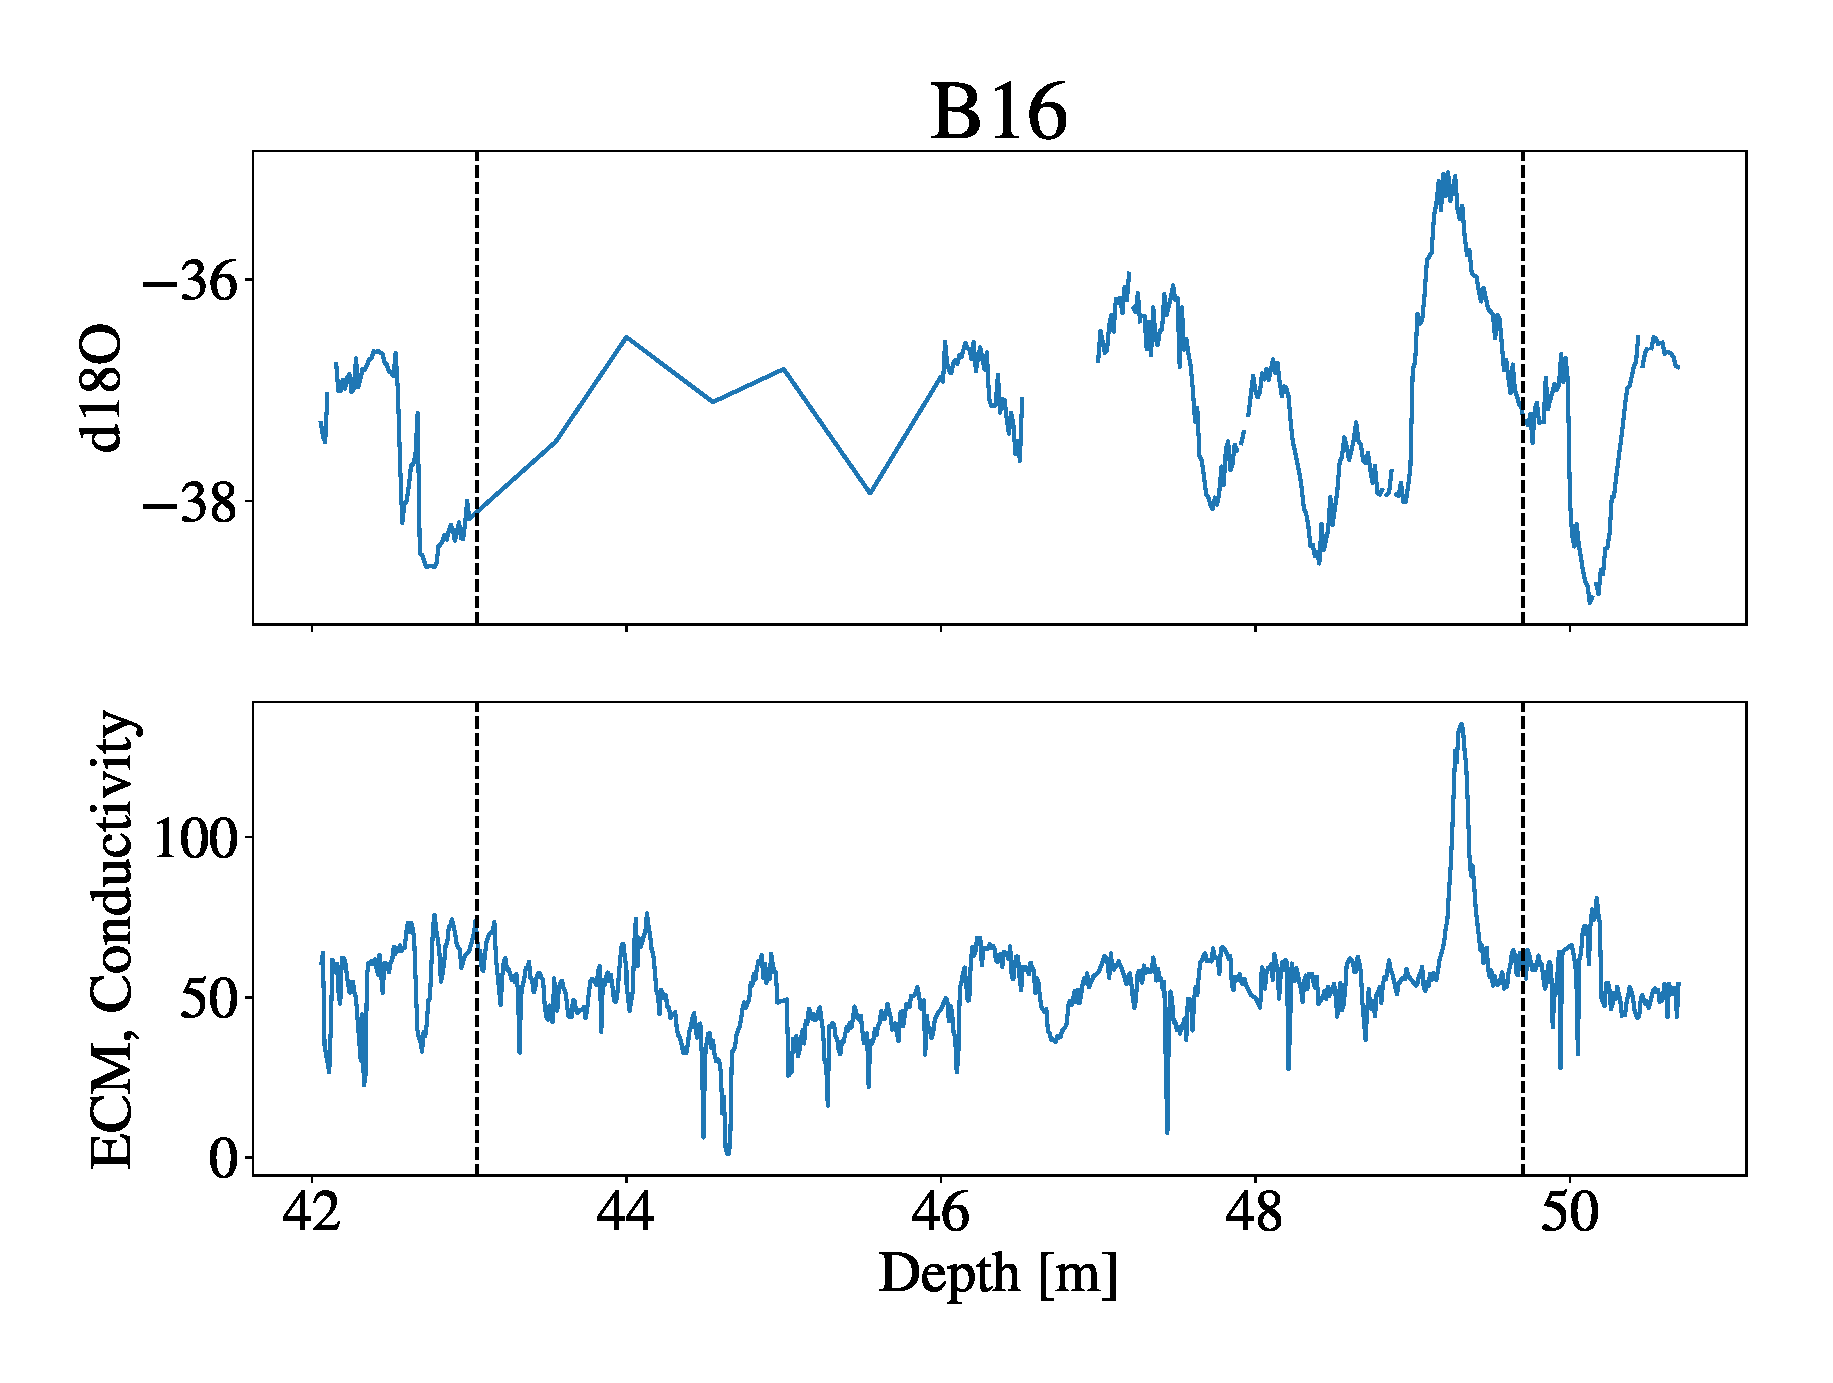
\includegraphics[width =0.3\linewidth]{Core_LT_B16.eps} & 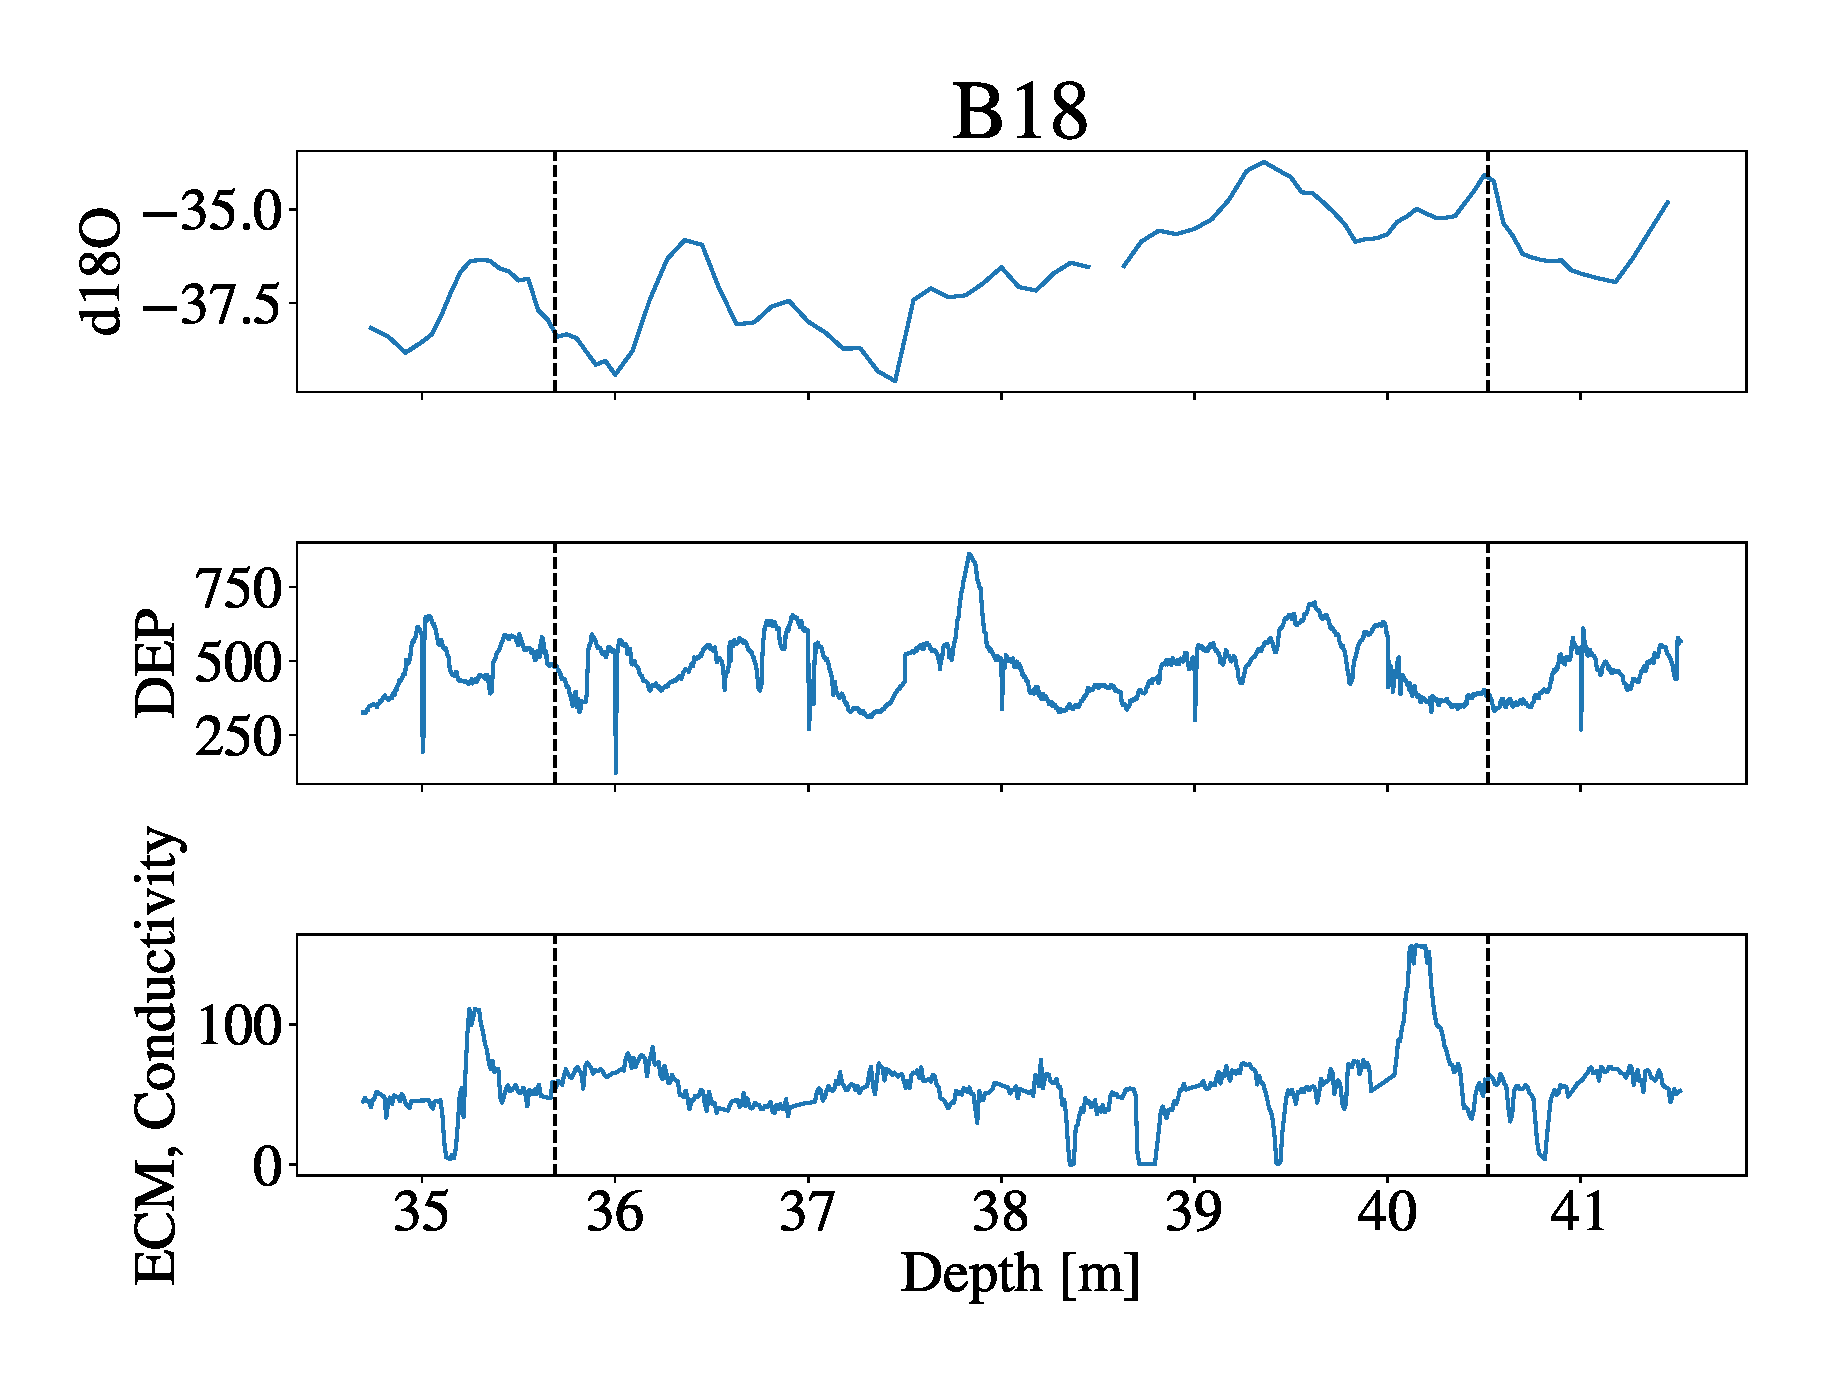
\includegraphics[width =0.3\linewidth]{Core_LT_B18.eps} & 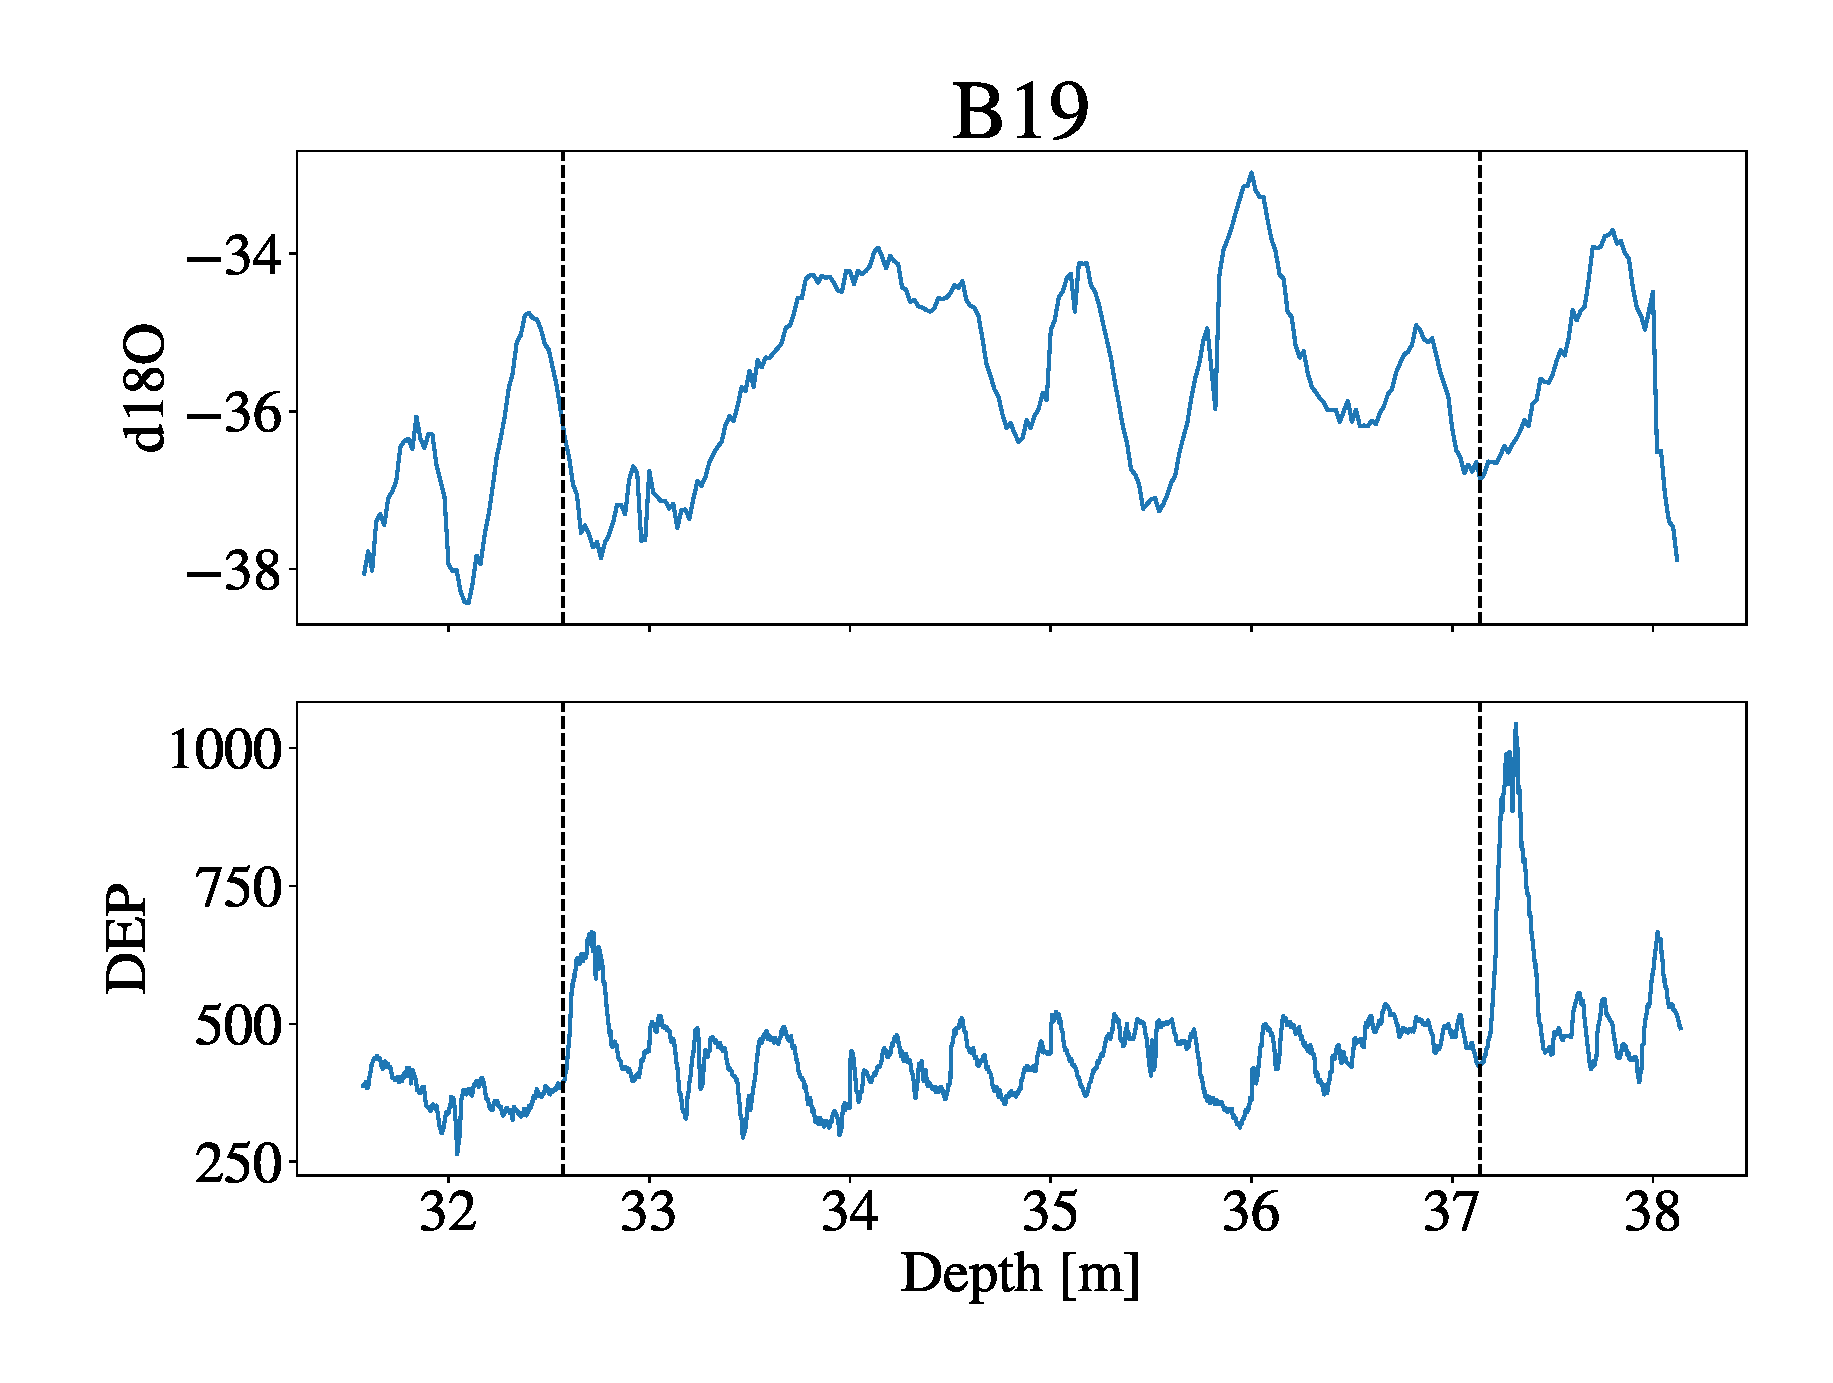
\includegraphics[width =0.3\linewidth]{Core_LT_B19.eps} \\
					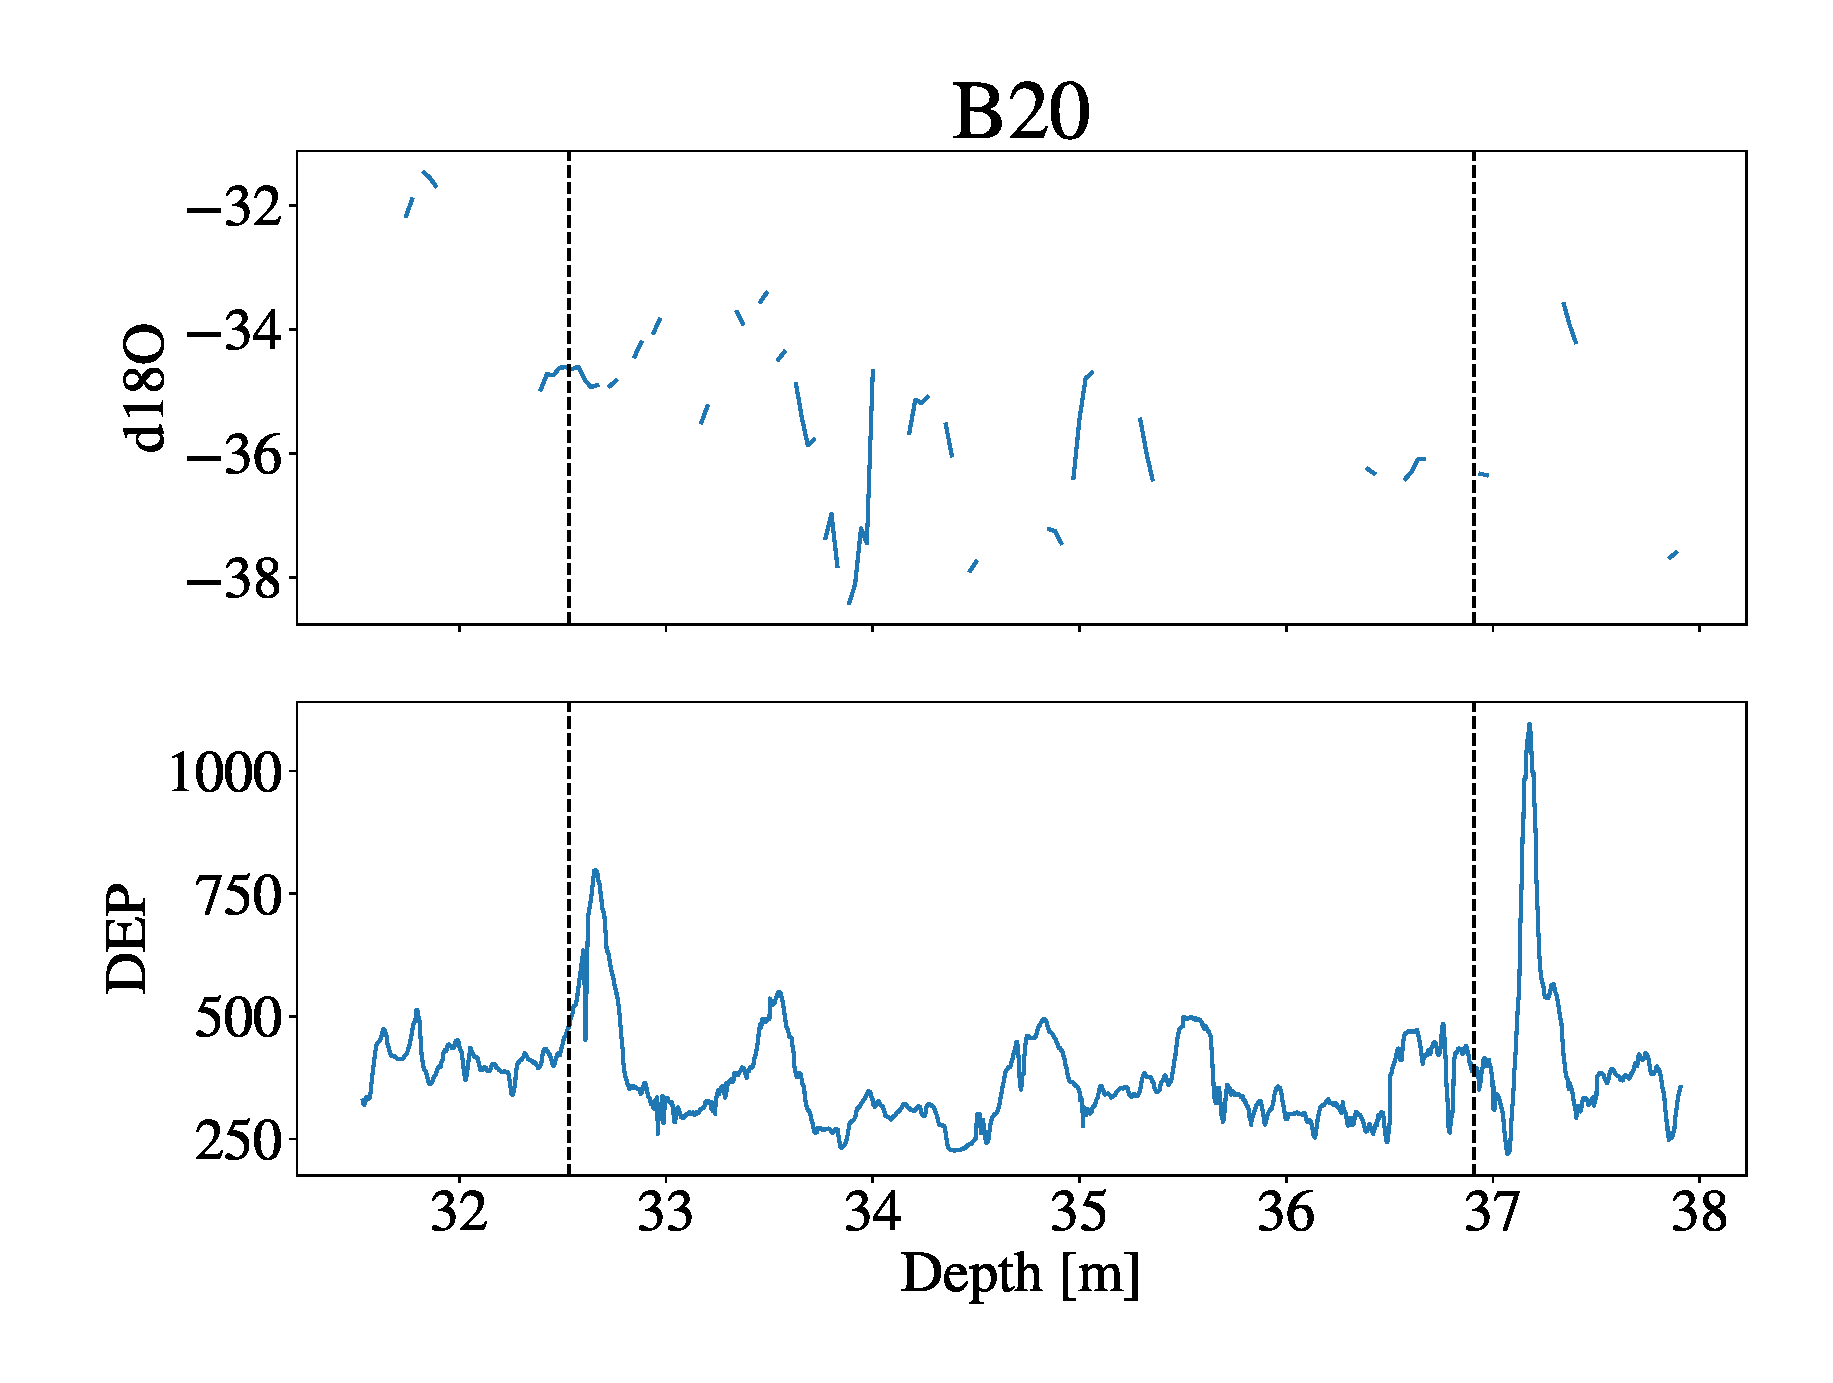
\includegraphics[width =0.3\linewidth]{Core_LT_B20.eps} & 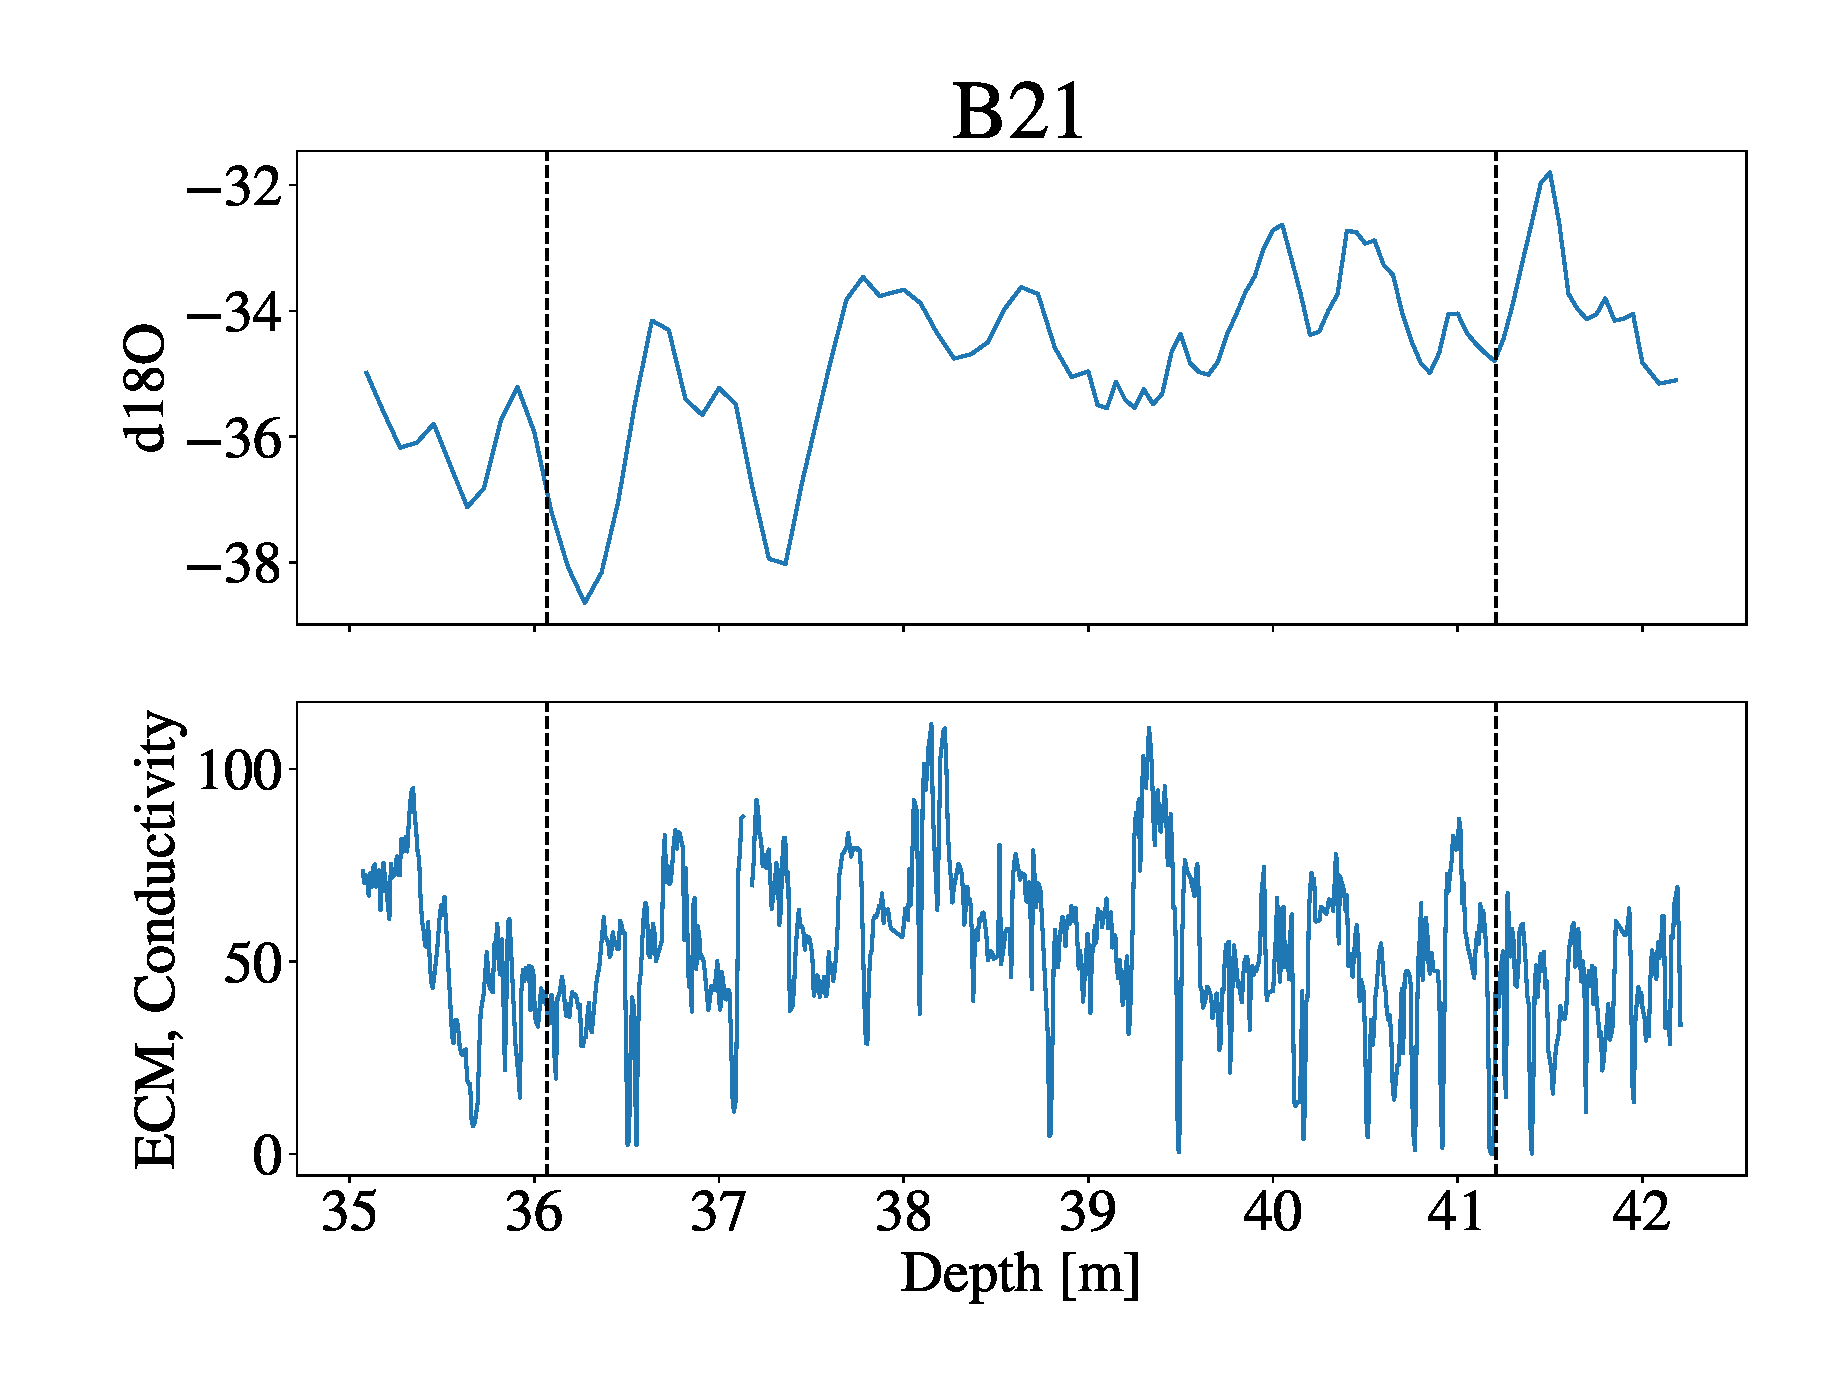
\includegraphics[width =0.3\linewidth]{Core_LT_B21.eps} & 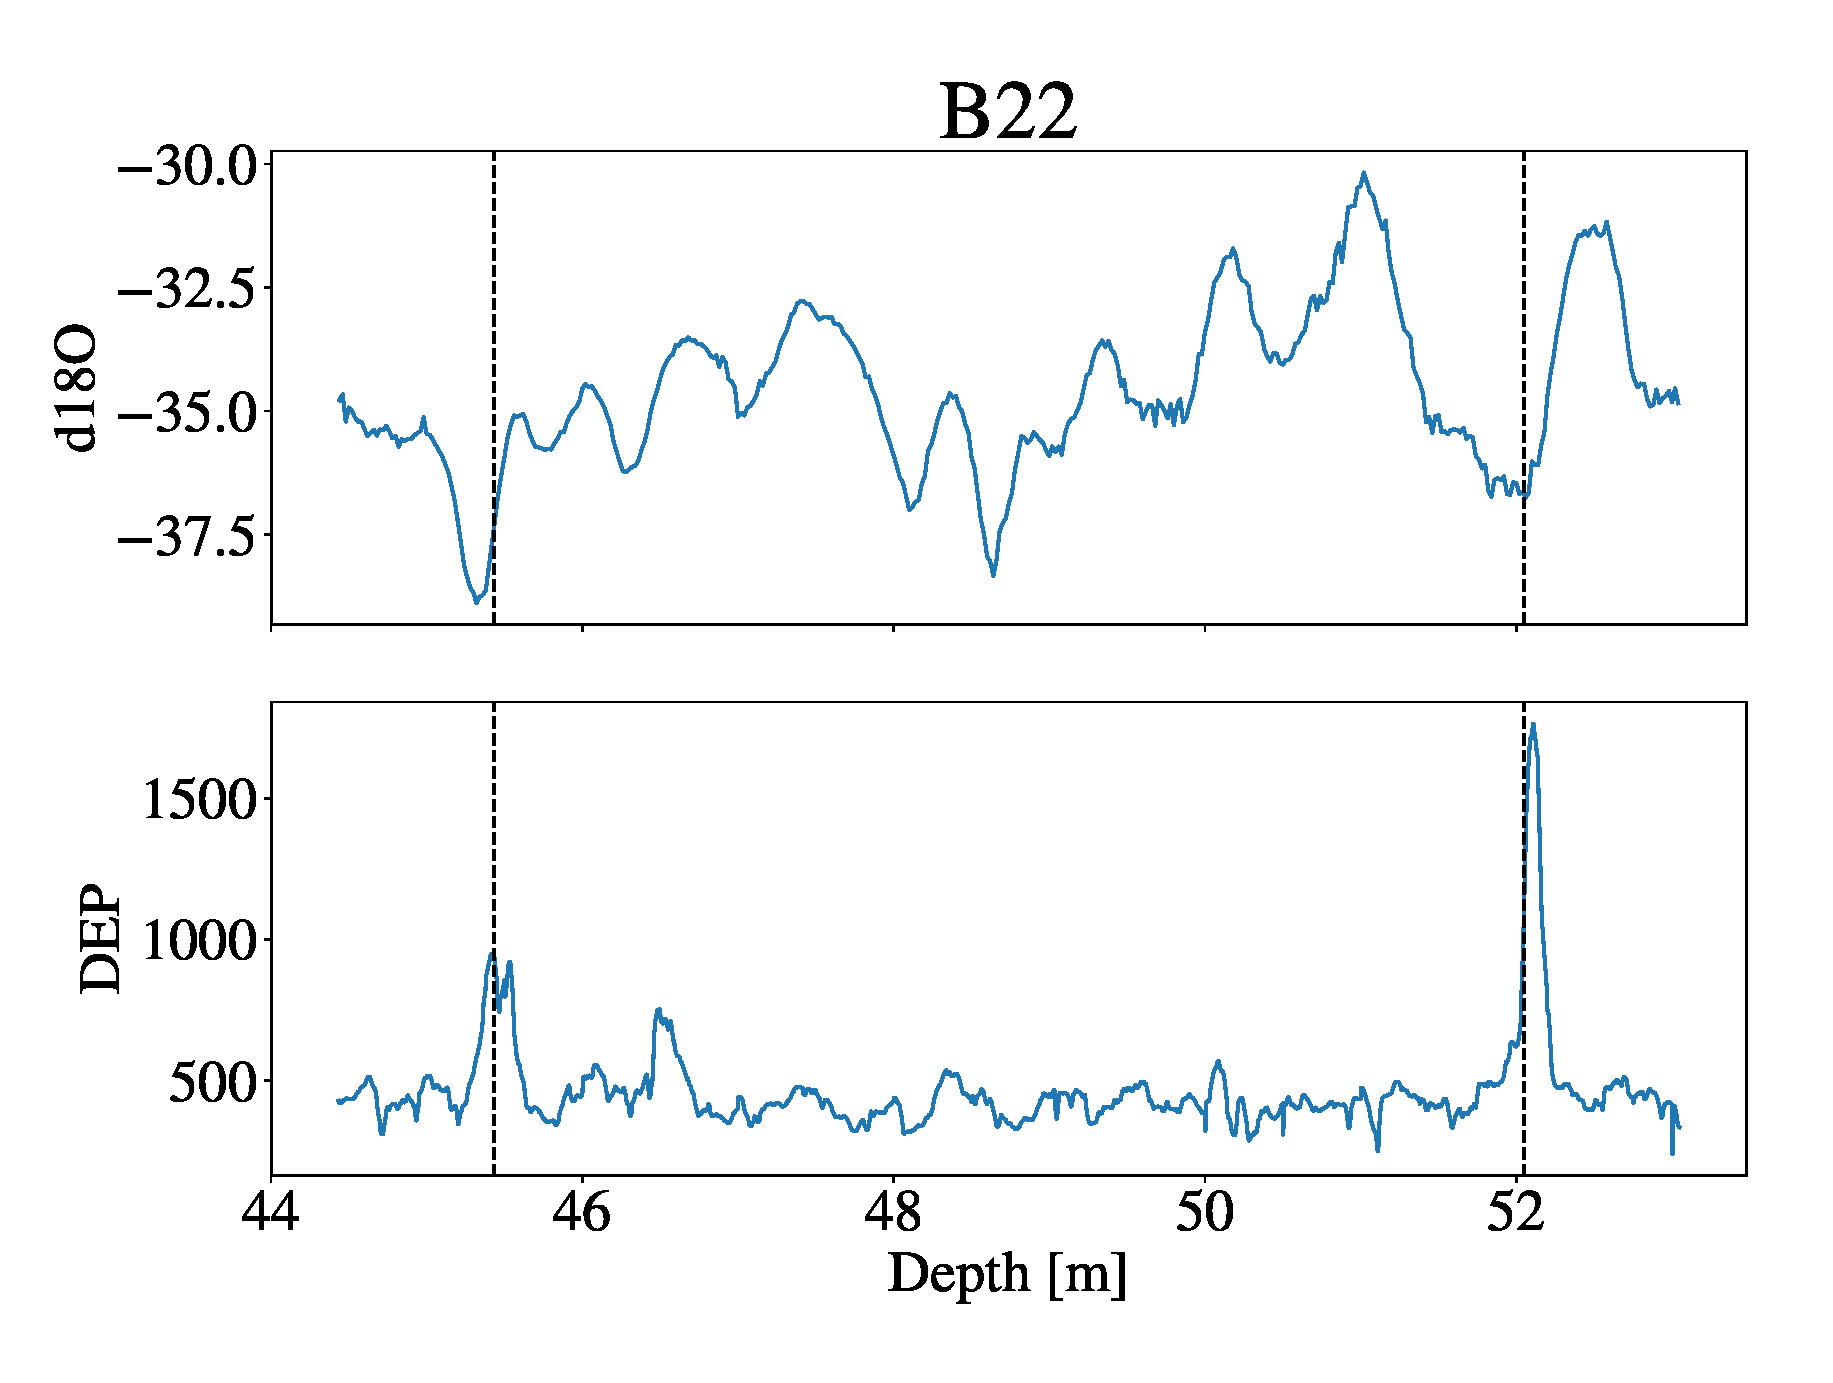
\includegraphics[width =0.3\linewidth]{Core_LT_B22.eps} \\	
					& & 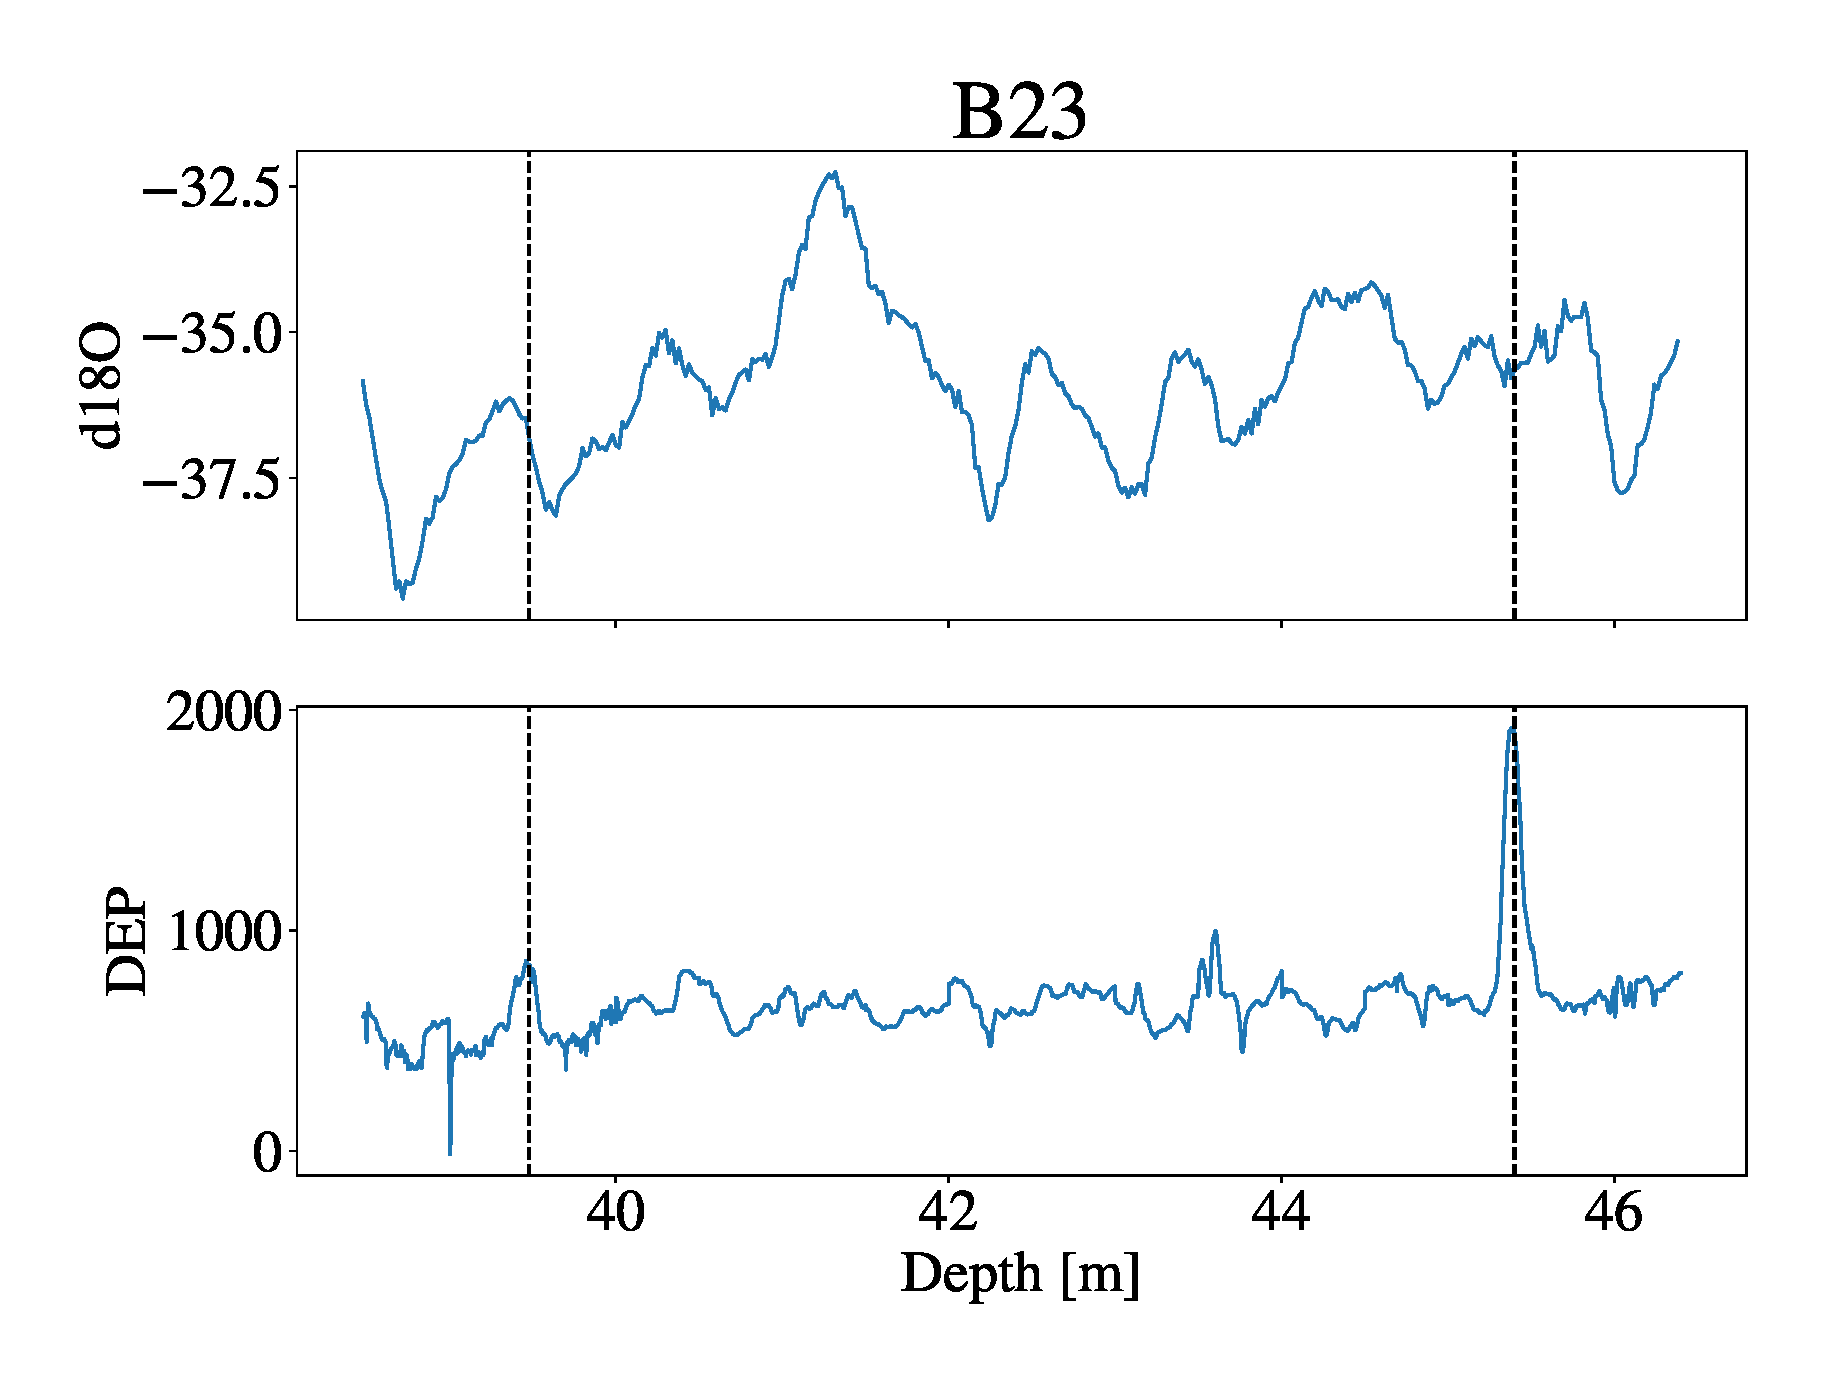
\includegraphics[width =0.3\linewidth]{Core_LT_B23.eps} \\
				\end{tabular}
			\end{table}
		\end{landscape}
	\end{rotatepage}
	\newpage
	
	\begin{rotatepage}
		\begin{landscape}
			\begin{figure}[h]
				\centering
				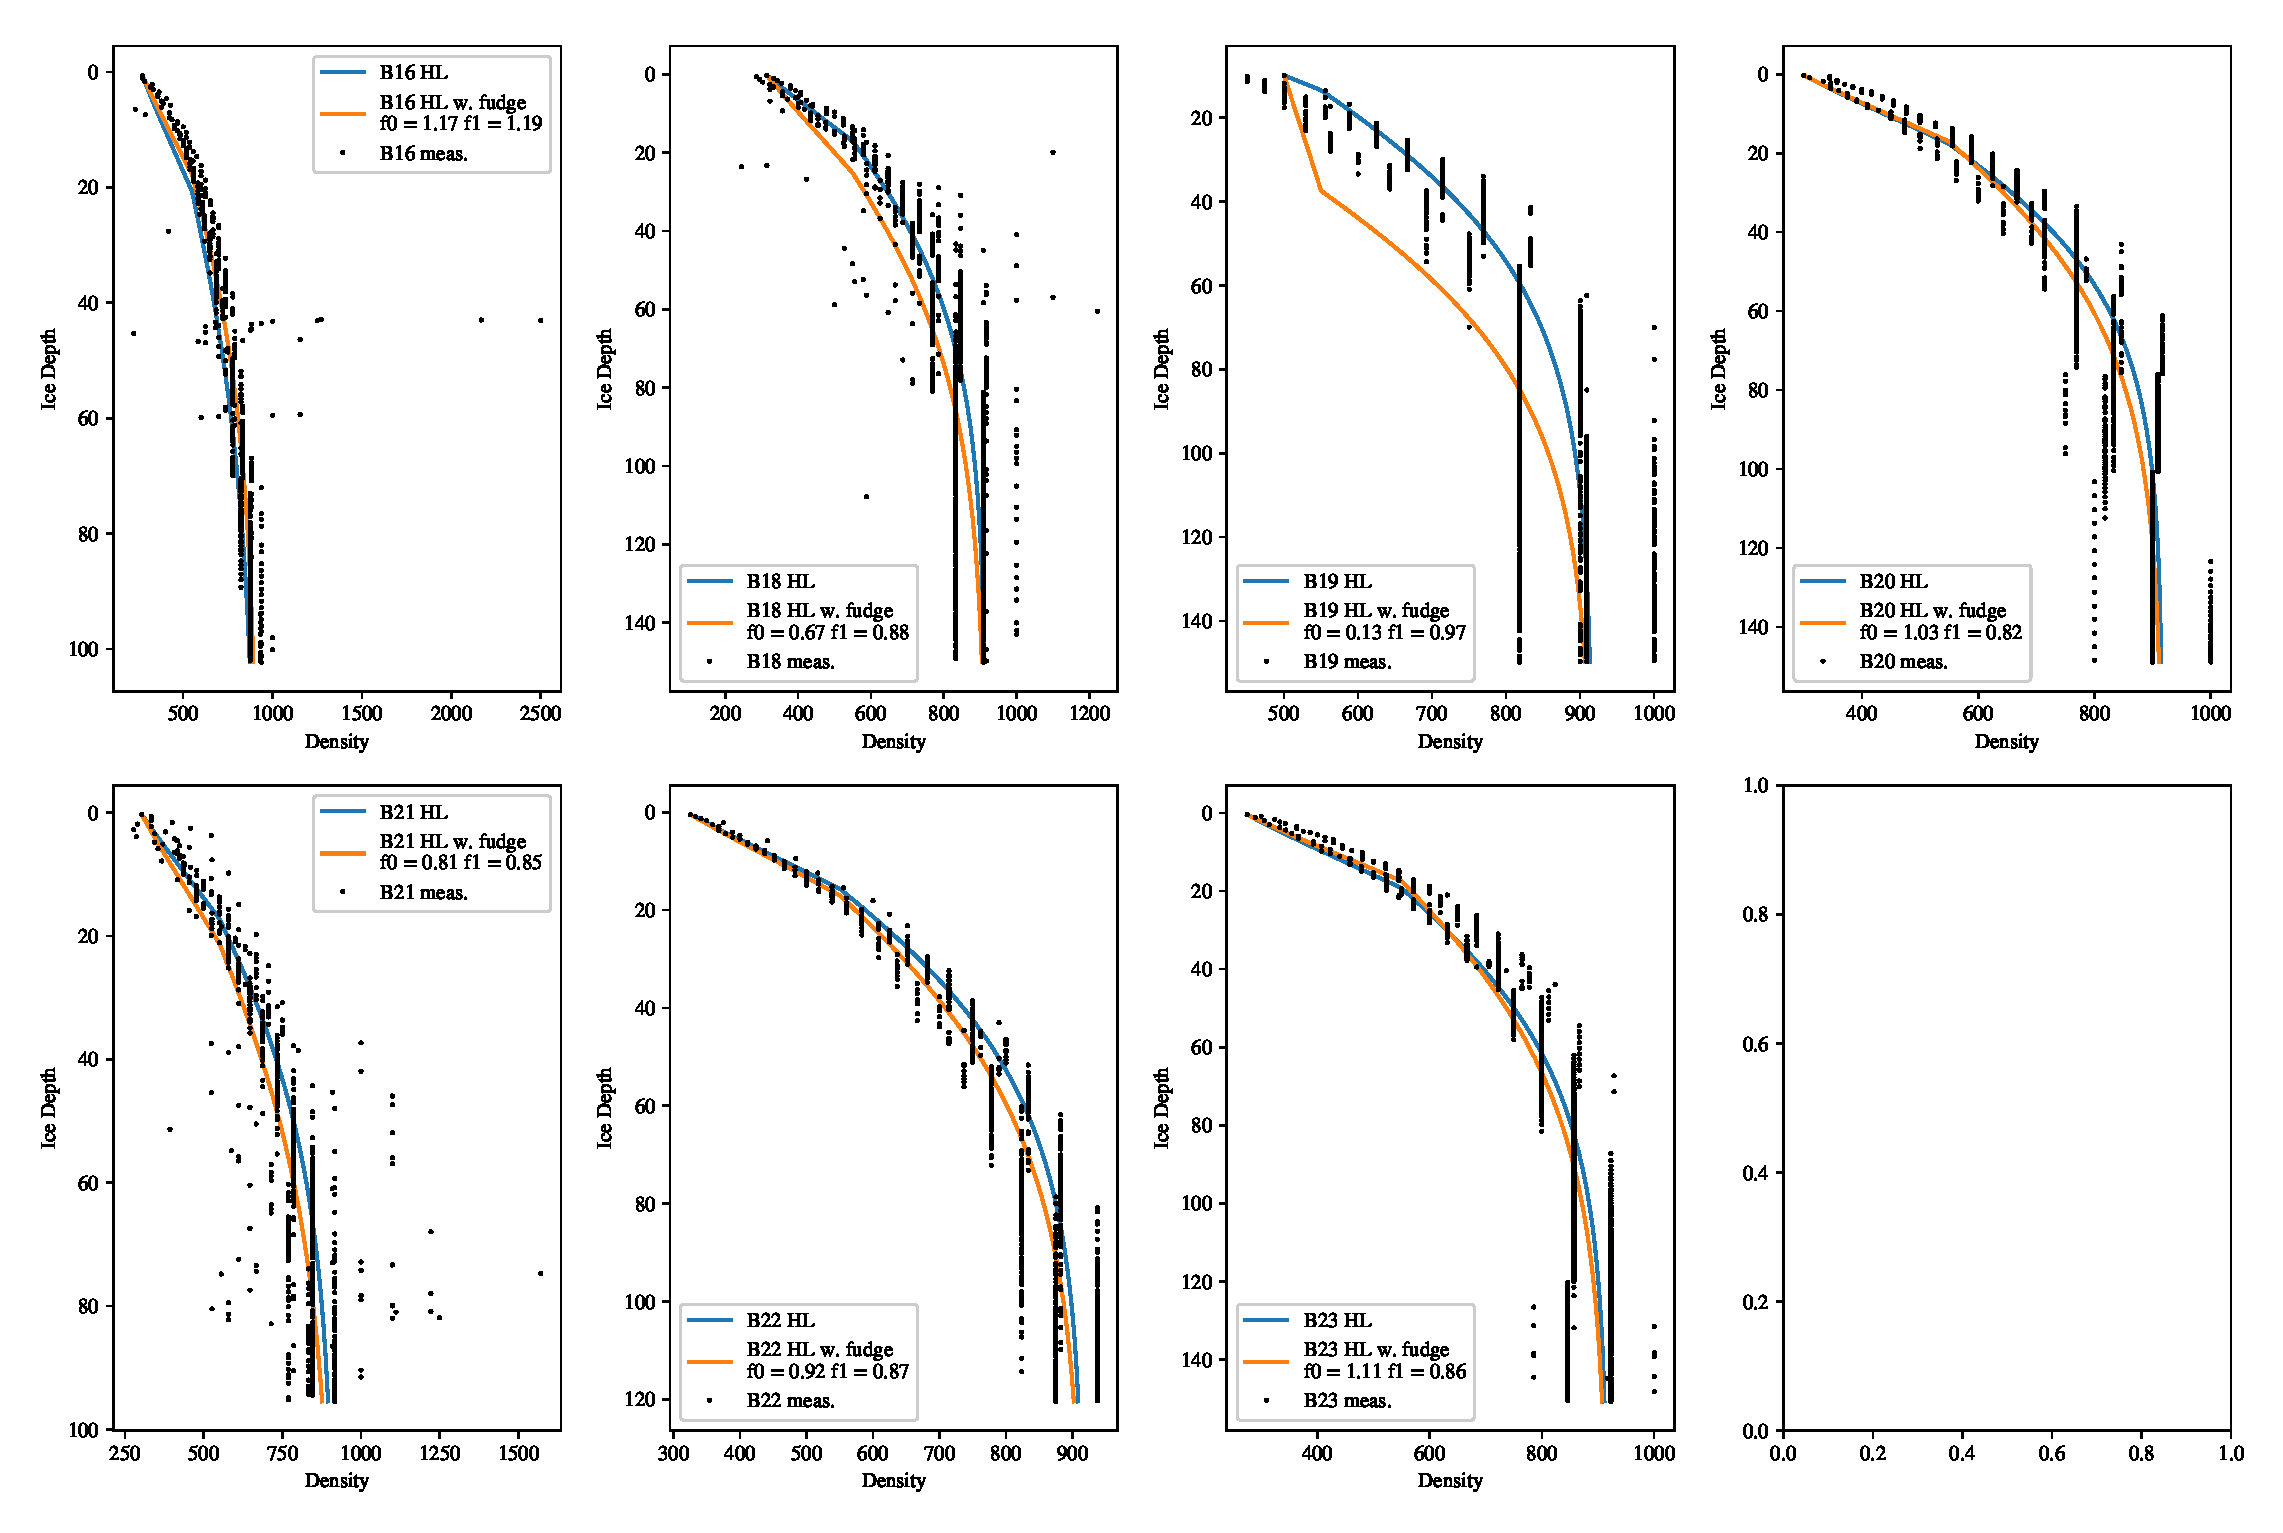
\includegraphics[width=1.5\textwidth]{fig_dens_B16B18B19B20B21B22B23.eps}
				\label{fig:dens}
				\caption{AWI B-cores density measurements and HL-modeled densities.}
			\end{figure}
		\end{landscape}
	\end{rotatepage}
	\newpage
	\begin{rotatepage}
		\begin{landscape}
			\begin{figure}[h]
				\centering
				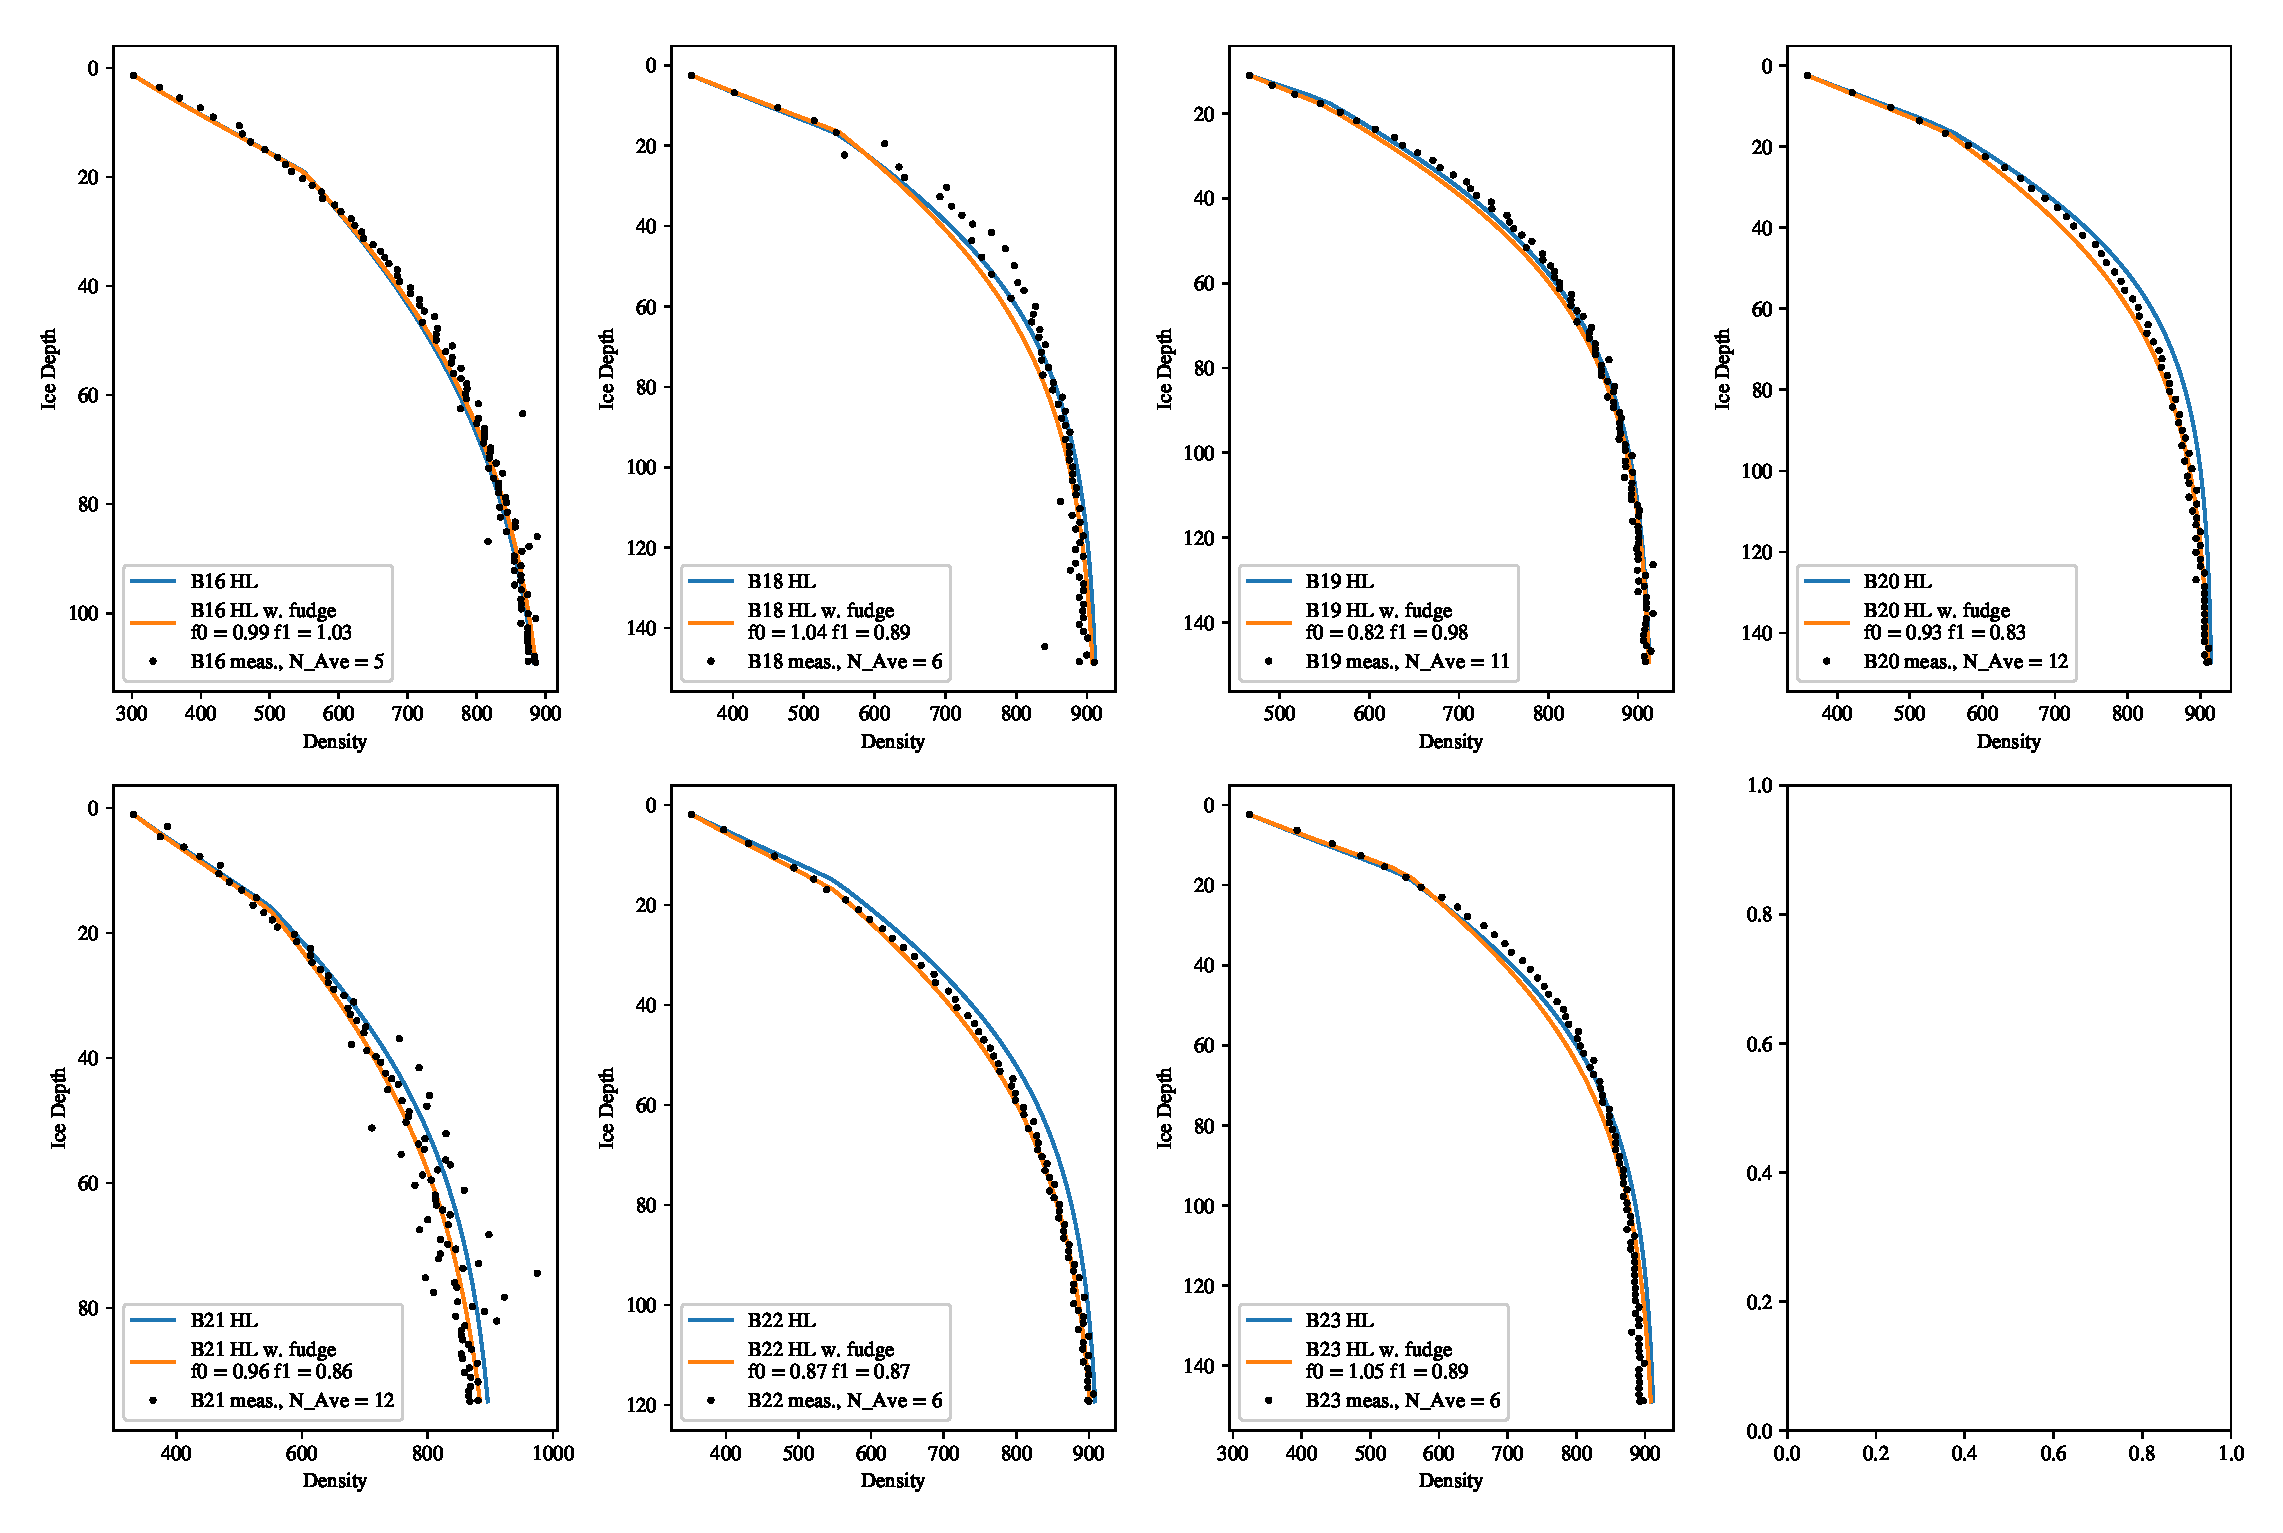
\includegraphics[width=1.5\textwidth]{fig_densAve_B16B18B19B20B21B22B23.eps}
				\label{fig:densAve}
				\caption{AWI B-cores averaged density measurements and related HL-modeled densities.}
			\end{figure}
		\end{landscape}
	\end{rotatepage}
	
	
	
	\newpage
	\section[Appendix III]{APPENDIX III: Data - Alphabet Cores}
	\label{AppIII:Data_Alphabet}
	\begin{figure}[h]
		\centering
		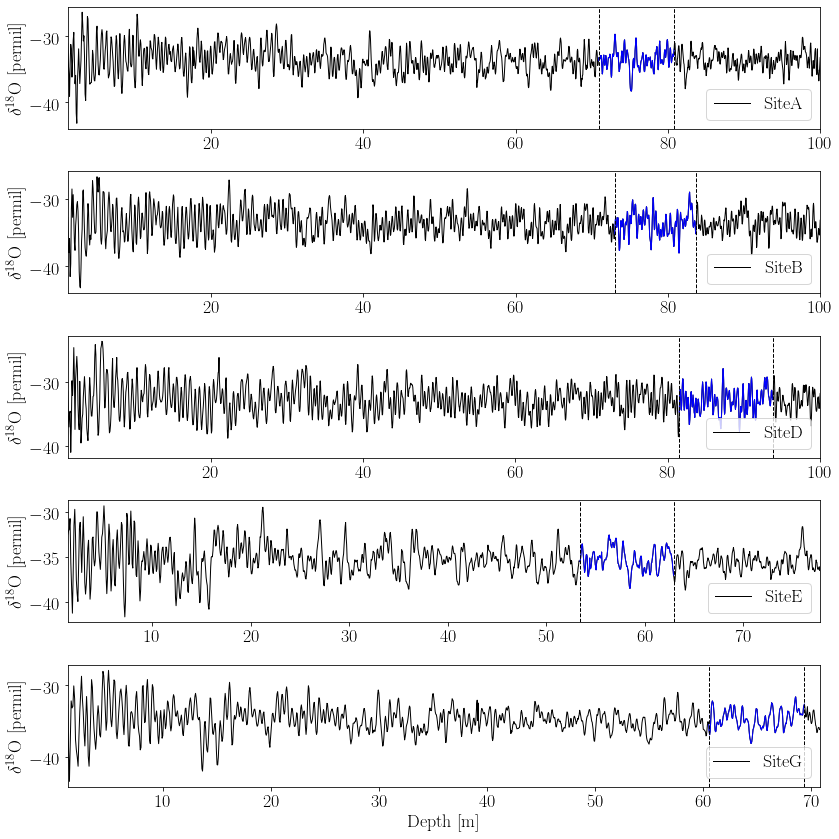
\includegraphics[width=0.9\textwidth]{AllAlphabetCores.png}
		\caption[]{All six Alphabet cores under examination, with Laki to Tambora depth section highlighted.}
		\label{fig:AllAlphabetCores}
	\end{figure}
	
	\begin{figure}[H]
		\centering
		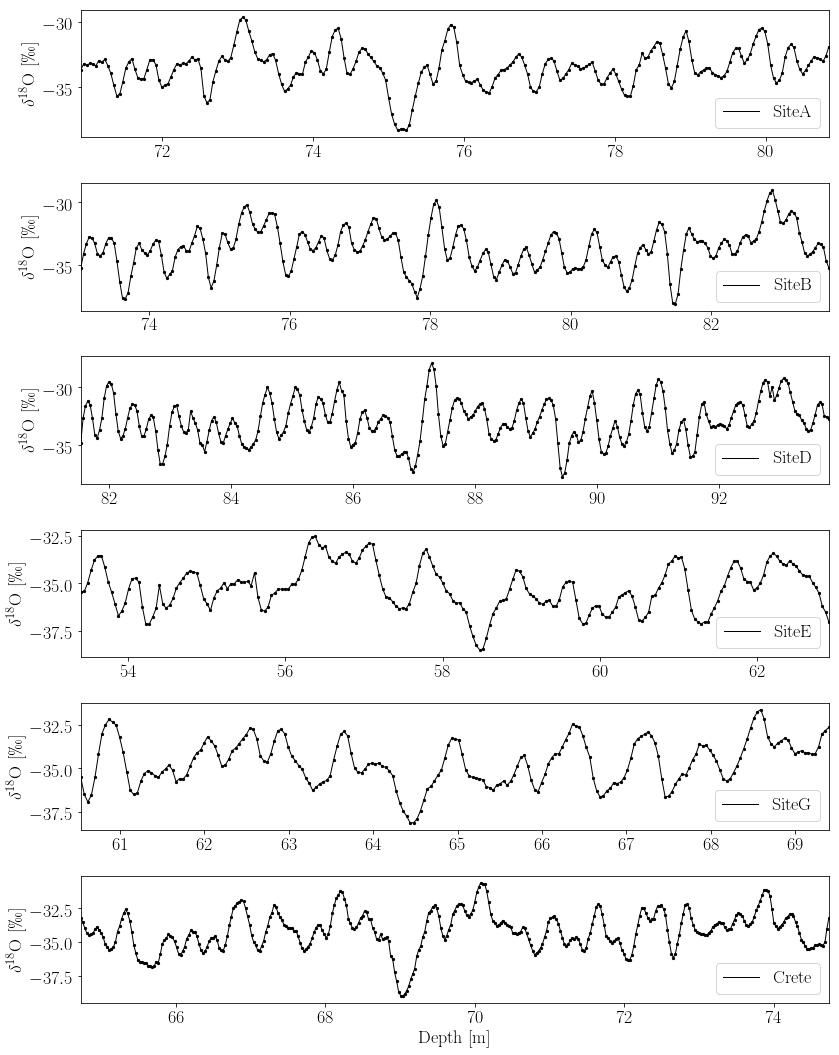
\includegraphics[width=\textwidth]{AllAlphabetCores_LT.png}
		\caption[]{All six Alphabet cores, showing only the depth series concerning the Laki to Tambora section.}
		\label{fig:AllAlphabetCores_LT}
	\end{figure}
	\newpage
	
	
	\newpage
	\section[Appendix IV]{APPENDIX IV: Spectral Transforms}
	\label{AppIV:SpectralTransforms}		
	\subsubsection[DFT \& FFT][DFT \& FFT]{Discrete and Fast Fourier Transform}
	\label{Subsubsec:SignalAnalysis_BackDiffusion_SpectralAnalysis_DFTFFT}
	The definition of the continuous Fourier transform and its inverse was presented in the above. The Fourier transform is as seen a way of representing the function under consideration as an infinite sum of periodic components. When the function is discrete, so will the Fourier transform be, and the integral is replaced with a sum. This gives us the Discrete Fourier Transform (DFT) which transforms the signal into a sum of separate components contributing at different frequencies. The DFT is dependent on the sampling interval, $\Delta$, and we can describe our discrete signal $X$ as a function of N discrete time steps $t_k = k\cdot\Delta$, where $k = 0, \, 1,\, ..., \, N-1$:
	\begin{equation}
		X_k \equiv X(t_k)
		\label{Eq:DiscreteSignal}
	\end{equation}
	This sample size is supposed to be representative for the entire discrete function, if the function continues beyond the $N$ sampled points. When sampling discretely at interval $\Delta$, there will be a special frequency, the Nyquist critical frequency, defined through the sampling size as:
	\begin{equation}
		f_{NQ} \equiv \frac{1}{2\Delta}.
		\label{Eq:NyquistFreq}
	\end{equation}
	This frequency is of great importance in transformation of discrete signals. If the continuous signal is sampled at an interval $\Delta$ is bandwidth limited to frequencies smaller in magnitude than $f_{NQ}$, $\tilde{X}(f) = 0 \text{ for } |f| \geq f_{NQ}$ - i.e. the transformed function has only non-zero values inside the Nyquist interval, $\tilde{X}(-f_{NQ}), ..., \tilde{X}(f), ..., \tilde{X}(f_{NQ})$. This means that the function is completely determined since we have all information about the signal contained in our available frequency space.\\
	On the other hand, which is much more likely, if the continuous signal consists of frequencies both inside and outside the Nyquist interval, then all spectral information outside of this range will be falsely interpreted as being inside this range. Thus a wave inside the interval with a frequency of $f_n$ will have a number of wave siblings outside of the interval, with frequencies  of $k\cdot \frac{1}{\Delta} f_n$, $k$ being integers, which will be aliased into the Nyquist interval and give rise to an increased power at the frequency $f_n$.\\
	When analyzing an already measured discrete signal, this might give rise to some headache. What can be done is to assume that the signal has been sampled competently and then assume that the Fourier transform is zero outside of the Nyquist interval. After the analysis it will then be possible to determine if the signal was indeed competently sampled, as the Fourier series will go to zero at $f_{NQ}$ given a correct assumption, and go to a fixed value, if the sampling was not done competently.\\
	Now with the basics of understanding the limits of frequency transform of a discretely sampled signal, it is possible to estimate the DFT of the signal $X_k \equiv X(t_k)$. Since the Fourier transform is a symmetric transformation it is easiest to assume that $N$ is even.
	
	Since the input information is of size $N$ we should expect only to sample the frequency transform $\tilde{X}(f)$ at only discrete values of f in the range between the upper and lower critical Nyquist frequencies, $-f_{NQ}$ to $f_{NQ}$:
	\begin{equation}
		f_n \equiv \frac{n}{N\Delta}, \qquad n = -\frac{N}{2}, ..., \frac{N}{2}
		\label{Eq:FreqNQRange}
	\end{equation}
	This will indeed actually give rise to $N+1$ values, since 0 will be in the interval as well, but the limit frequencies are actually not independent, but all frequencies between are, which reduces it to $N$ samples. \\
	Now the integral from Equation \ref{Eq:FourierTransform} needs to be estimated as a sum:
	\begin{equation}
		\tilde{X}(f_n) = \int_{-\infty}^{\infty} X(\tau) e^{2\pi i f_n \tau} dt \approx  \sum_{k=0}^{N-1}X_k e^{2\pi i f_n t_k} \Delta = \Delta \sum_{k=0}^{N-1}X_k e^{2\pi i k \frac{n}{N}}
		\label{Eq:DFTestimation}
	\end{equation}
	The Discrete Fourier Transform is thus defined as:
	\begin{equation}
		\tilde{X}_n \equiv  \sum_{k=0}^{N-1}X_k e^{2\pi i k \frac{n}{N}}
		\label{Eq:DFT}
	\end{equation}
	This gives the approximate relation between the DFT estimate and the continuous Fourier transform $\tilde{X}(f)$ when sampling at size $\Delta$ as:
	\begin{equation}
		\tilde{X}(f_n) \approx \Delta \tilde{X}_n
	\end{equation}
	The inverse DFT is given as:
	\begin{equation}
		X_n \equiv \frac{1}{N} \sum_{n=0}^{N-1}X\tilde{X}_n e^{-2\pi i k \frac{n}{N}}
		\label{Eq:InverseDFT}
	\end{equation}
	Computation of the DFT can be very slow and tiresome, since it involves complex multiplication between a number of vectors and matrices. If we write Equation \ref{Eq:DFT} as $\tilde{X}_n = \sum_{k=0}{N-1}W^{nk}X_k,$ where  $W$ is a complex number $W\equiv e^{2\pi i /N}$. This shows that the vector $X_k$ must be multiplied with a complex matrix which (n,k)th component consists of the constant $W$ to the power of $nk$. This matrix multiplication evidently leads to a process of $O(N^2)$. Fortunately, a number of different algorithms implementing a wide range of different theories from complex number arithmetic and prime-factoring to group and number theory (\cite{Cooley1965},\cite{Good1958_PrimeFFT}, \cite{Bruun1978__BruunsFFT} and others) have been developed for fast and efficient computation of the discrete Fourier transform. One of these is called the Fast Fourier Transform (FFT), which can reduce the computations to just $\mathcal{O}(N\log_2 N)$. In this thesis the FFT used is the one implemented in the \lstinline[language=Python]|scipy.fft| Python package \cite{Virtanen2020_SciPy}, which is based on the works of \cite{Cooley1965}. See said article for implementation details. One important thing about this specific algorithm is that for the algorithm to function most efficiently, the number of points computed in the frequency space must be of a power of 2, following the use of base $\log_2$
	
	\subsubsection[NUFT][NUFT]{Nonuniform Discrete Fourier Transform}
	\label{Subsubsec:SignalAnalysis_BackDiffusion_SpectralAnalysis_NUFT}
	All FFT algorithms evaluates the DFT definitions from Eqs. \ref{Eq:DFT} to \ref{Eq:InverseDFT} in fast and efficient ways. But one key assumption for these methods is that the data under examination are equispaced, i.e. uniformly distributed, based on the summation in Eq. \ref{Eq:DFT}. The computations thus expect uniform data as input and returns uniform data as output. Unfortunately this is not always the case for data collected in physical experiments. In this case the basic assumptions for the calculations of both DFT and FFT are flawed. \\
	The most general form of a nonuniform transform would be the one that takes non-equispaced data as input and also returns non-equispaced transforms as output. Firstly we wish to create a nonuniform discrete Fourier transform (NUDFT) that transforms a sequence of $N$ complex numbers $X_0,...,X_{N-1}$ to a different sequence of $M$ complex numbers, $\tilde{X}_0,...,\tilde{X}_{M-1}$. The one-dimensional NUDFT the computes the transformed vector $\tilde{\boldsymbol{X}} = (\tilde{X}_0,...,\tilde{X}_{M-1})^{\text{T}}$, with entries computed as the sum
	\begin{equation}
		\tilde{X}_k = \sum_{n=0}^{N-1} X_n e^{-2\pi i p_n f_k},\qquad 0 \leq k \leq M-1.
		\label{Eq:NDFT} 
	\end{equation}
	The values $X_0, ...,X_{N-1}$ are sample values, $p_0,...,p_{N-1}$ are sample positions and $f_0,...,f_{M-1}$ are frequencies. The NUDFT vector $\tilde{\boldsymbol{X}}$ is found by computing $M$ sums with each $N$ terms. This meaning that the computational cost will be of order $\mathcal{O}(M\cdot N)$, and if $M=N$ then of $\mathcal{O}(N^2)$. The NUDFT reduces to the DFT if the points are equispaced, $p_n = \frac{n}{N}$, and the frequencies are integers, $f_k = k$, and can be computed at the cost of the FFT, $\mathcal{O}(N\log_2 N)$. In the literature there are many who have presented different ways to develop a fast NUDFT (\cite{Potts2001}, \cite{Marvasti1993}, \cite{Ruiz-Antolin2018}, \cite{Lee2005} among others), generally referred to as NUFFT or NFFT. In this work though, the main focus is on the discrete cosine transform, and the NFFT methods will not be described in depth\\
	
	
	\subsubsection[DCT][DCT]{Discrete Cosine Transform}
	\label{Subsubsec:SignalAnalysis_BackDiffusion_SpectralAnalysis_DCT}
	The Fourier transform in any of its many forms is designed to process complex-valued signals, always producing a complex-valued spectrum, even for signals that were strictly real-valued. The real-valued or complex-valued part of the Fourier spectrum is on their own not enough to represent the full information of the signal, since neither the cosine nor he sine functions (corresponding to the real and the complex parts of the spectrum respectively), constitute a complete set of basis functions. Nonetheless, a purely real-valued signal has a symmetric Fourier spectrum, meaning that it is only necessary to compute half the number of spectral coefficients, without losing any signal information. Since the signals analyzed in this thesis are strictly real, one way to use this knowledge to improve on the works of this project is to consider a different, less expensive, purely real spectral transform. The cosine transform \cite{Ahmed1974_DCT} seems to do the trick: it uses only cosine functions as basis functions and operates with only real-valued signal and spectral coefficients, and have properties similar to the Fourier transform.\\
	For the discrete version of the cosine transform, DCT, and its inverse, IDCT, a number of different definitions have been proposed, but for this work, the originally formulations by \cite{Ahmed1974_DCT} are used. These are often referred to as "The DCT" and "The IDCT", and other times as DCT-II and DCT-III. The entries of the computed discrete cosine transform vector,$\tilde{X}_0,...,\tilde{X}_{M-1}$ , of a real-valued signal of $N$ data points, $X_0,...X_{N-1}$, is computed as
	\begin{equation}
		\tilde{X}_k = 2\sum_{n=0}^{N-1} X_n \cos\left(\frac{\pi(2n+1)k}{2N}\right),\qquad 0\leq k < M.
		\label{Eq:DCT}
	\end{equation}
	
	To orthonormalize the base functions,$\phi_k(n)$ , the coefficients are multiplied by a scaling factor $f$:
	\begin{equation}
		f = \begin{cases}
			\frac{1}{\sqrt{2N}}, & \text{if} k = 0 \\
			\frac{1}{\sqrt{4N}}, & \text{otherwise}
		\end{cases}
		\label{Eq:DCT_OrthoScalingFactor}
	\end{equation}
	so that the base functions, $\phi_k[n] = 2f\cos\left(\frac{\pi(2n+1)k}{2N}\right)$, meet the condition:
	\begin{equation}
		\sum_{n=0}^{N-1} \phi_k[n]\phi_l[n] = \delta_{lk}.
		\label{Eq:DCT_Orthonormalization}
	\end{equation}
	
	The inverse of the DCT, the so called DCT-III, is defined, unnormalized, as: 
	\begin{equation}
		X_k = \tilde{X}_0 + 2\sum_{n=1}^{N-1} \tilde{X}_n\cos\left(\frac{\pi n(2k+1)}{2N}\right), \qquad 0 \leq k < N 
		\label{Eq:IDCT}
	\end{equation}
	and orthonormalized:
	\begin{equation}
		X_k = \frac{\tilde{X}_0}{\sqrt{N}} + \sqrt{\frac{2}{N}}\sum_{n=1}^{N-1} \tilde{X}_n\cos\left(\frac{\pi n(2k+1)}{2N}\right), \qquad 0 \leq k < N 
		\label{Eq:IDCT_ortho}
	\end{equation}
	
	Only when the DCT-III is orthonormalized is it exactly the inverse of the orthonormalized DCT-II. If they are both unnormalized, the DCT-III is the inverse of the DCT-II up to a factor $2N$.
	As with the DFT, the DCT can directly be computed at a cost of $\mathcal{O}(N\cdot M)$, and can also reduced to $\mathcal{O}(N \log N)$. The fast DCT algorithm(FCT) used here is based on \cite{Makhoul1980} as it is implemented in the \lstinline[language=Python]|scipy.fft.dct| package\cite{Virtanen2020_SciPy}.
	
	\subsubsection[NDCT][NDCT]{Nonuniform Discrete Cosine Transform}
	\label{Subsubsec:SignalAnalysis_BackDiffusion_SpectralAnalysis_NDCT}
	Again, as with the FFT, the FCT works under the key assumption that data is equispaced. Though when data is nonuniform, the DCT is described as:
	\begin{equation}
		\tilde{X}_k = 2\sum_{n=0}^{N-1}X_n \cos\left(2\pi f_k\left(p_n + \frac{1}{2N}\right)\right), \qquad 0 \leq k < M-1
		\label{Eq:NDCT}
	\end{equation}
	with, in the most general case, nonuniformly spaced signal, $p_o,...,p_{N-1}$, data and frequency data, $f_0,...,f_{M-1}$.
	The inverse of NDCT, the INDCT, is computed as:
	\begin{equation}
		X_k = \frac{\tilde{X}_0}{\sqrt{N}} + \sqrt{\frac{2}{N}}\sum_{n=1}^{N-1} \tilde{X}_n \cos\left(\left(p_n + \frac{1}{2N}\right)2\pi f_k\right), \qquad 0 \leq k < N -1
		\label{Eq:INDCT}
	\end{equation}
	
	It is possible to develop algorithms with the computational cost of $\mathcal{O}(N\log N)$ for NDCT and INDCT as it is for 
	the NDFT (\cite{Tian2000}, \cite{Zhao2008}) but it has showed to be out of the scope of this project and has not been implemented. This of course slows down the final optimization algorithm, as it requires a number of spectral transformations. In Section \ref{Sec:Method} it is described how the final algorithm has been designed to minimize the use of NDCT, and thus speeding up the final computations.
	
	
	\subsubsection[MEM][MEM]{Maximum Entropy Method (Burg's Method)}
	\label{Subsubsec:SignalAnalysis_BackDiffusion_SpectralAnalysis_MEM}
	\todo{SIGNAL-MEM: Write this entire section - maybe not necessary? Maybe use in reconstruction of missing data...}
	
	
	
	\newpage
	\section[Appendix V]{APPENDIX V: Splines and Interpolations}
	\label{AppV:SplinesAndInterpolation}
	
	\subsubsection[Existence and Uniqueness]{Existence, Uniqueness and Conditioning}
	Considering any attempt to create an interpolant to fit a number of data points, the questions of uniqueness and existence is a matter of matching the data points with the number of parameters in the interpolant. If there are too few parameters, the interpolant does not exist, as it will not pass through all data points. If there are too many, the interpolant will not be unique. Formally this can be described through a system of linear equations.\\
	For any data set consisting of $(t_i, y_i),\; i=1,...,m$ points, an interpolant can be chosen from a function space spanned by some suitable set of basis functions, $\phi_1(t),...,\phi_n(t)$. The interpolant can then be described as a linear combination of these basis functions:
	\begin{equation}
		f(t) = \sum_{j=1}^{n} x_j\phi_j(t)
	\end{equation}
	The interpolant can then be found by determining the parameters $x_j$ by requiring that the interpolant $f$ must pass through the $M$ data points $(t_i,y_i)$:
	\begin{equation}
		f(t_i) = \sum_{j=1}^{n} x_j\phi_j(t_i) = y_i, \quad i=1,...,m
	\end{equation}
	This can of course also be written compactly in matrix form as a system of linear equations:
	\begin{equation}
		\boldsymbol{A}\boldsymbol{x}=\boldsymbol{y}
	\end{equation}
	In this equation $\boldsymbol{A}$ is the $m\times n$ basis matrix, which entries consists of the value of the $n$ basis functions evaluated at the $m$ data points, $a_{ij}=\phi_j(t_i)$, the $m$ vector $\boldsymbol{y}$ consists of the known data values $y_i$, and the $n$ vector $\boldsymbol{x}$ consists of the unknown, to be determined, parameters $x_j$.\\
	From linear algebra we know, that if we choose the number of basis function ot be equal to the number of data points, $n=m$, the basis matrix will be square, and thus - given the matrix is nonsingular - the system will be determined, and the data points can be fit exactly. Though in some problems it is beneficial to choose the system to be either overdetermined(less parameters than data points, the data cannot be fit exactly) or underdetermined(more parameters than data points, giving freedom to allow satisfaction of additional properties or conditions).\\ 
	So the existence and uniqueness of an interpolant is given by the non-singularity of the basis matrix, be it square or not and the conditioning of the matrix points to the parameters' sensitivity to perturbations. An ill-conditioned basis matrix will lead to high sensitivity in the parameters, but this problem can still be approximately solvable through Gaussian elimination with partial pivoting, but this solution will mean that the coefficients may be poorly determined.
	
	\subsubsection[Polynomial]{Polynomial Interpolation}
	\label{Sec:CompMeths_SplinesAndInterpolation_Interpolation_Polynomial}
	The most common way to determine an interpolant is through polynomials. Denoting a set of all polynomials of degree at most $k,\quad k\geq 0$ as $\mathbb{P}_k$, it can be seen that this set forms a vector space of dimension $k+1$. The basis functions that span this vector space can be chosen to be composed of a number of different functions and this choice has a great influence on both the cost of computation and manipulation of the interpolant, and the sensitivity of the parameters, i.e. the conditioning of the basis matrix. \\
	Considering $n$ data points it is obvious to choose $k=n-1$ so that the dimension of the vector space matches the number of data points. The maybe most natural choice of basis for $\mathbb{P}_{n-1}$ is one that consists of the first $n$ monomials\footnote{Roughly speaking, a polynomial with only one term.},
	\begin{equation}
		\phi_j(t) = t^{j-1},\quad j=1,...,n.
	\end{equation}
	Thus any given polynoial $p_{n-1}\in\mathbb{P}_{n-1}$ will be of the form 
	\begin{equation}
		p_{n-1}(t)=x_1 + x_2t + \cdots+x_n t^{n-1}.
	\end{equation}
	In this basis the system of $n\times n$ linear equations will be of the form 
	\begin{equation}
		\boldsymbol{A}\boldsymbol{x} = 
		\begin{bmatrix}
			1 & t_1 & \cdots & t_1^{n-1}\\
			1 & t_1 & \cdots & t_1^{n-1}\\
			\vdots & \vdots & \ddots & \vdots \\
			1 & t_1 & \cdots & t_1^{n-1}\\
			
		\end{bmatrix}
		\begin{bmatrix}
			x_1\\
			x_2\\
			\vdots\\
			x_n
		\end{bmatrix}
		=
		\begin{bmatrix}
			y_1\\
			y_2\\
			\vdots\\
			y_n
		\end{bmatrix}
		= \boldsymbol{y}.
	\end{equation}
	This type of matrix with geometric progression, i.e. the columns are successive powers of some independent variable $t$ is called a \todo{COMP-INTERP: REFERENCE!!!}Vandermonde matrix. \\
	When using the monomial basis and using a standard linear equation solver to determining the interpolants coefficients requires $\mathcal{O}(n^3)$ work and often results in ill-conditioned Vandermonde matrices $\boldsymbol{A}$, especially for high-degree polynomials. This ill-conditioning is due to the monomials of higher and higher degree being more and more indistinguishable from each other. This makes the columns of $\boldsymbol{A}$ nearly linearly dependent, resulting in almost singular matrices, and thus highly sensitive coefficients. For high enough $n$, the Vandermonde matrix becomes efficiently singular, to computational precision at least, though, as mentioned, this can be worked around, but requires some additional computational work. 
	
	\begin{marginfigure}
		\centering
		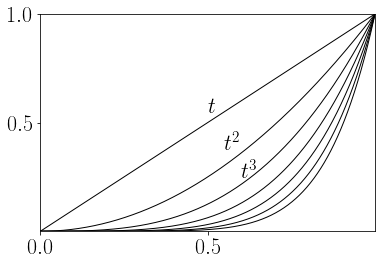
\includegraphics[width=\marginparwidth]{Monomials.png}
		\caption[Monomials]{\footnotesize{Illustration of the first eight monomials.}}% Black is the measured densities during drilling, blue is the modelled density profile given a Herron Langway model, and orange is a Herron Langway model with a criterion to minimize the distance to the actual measurements.}}
		\label{fig:Monomials}
	\end{marginfigure}
	\subsubsection[Piecewise Polynomial]{Piecewise Polynomial Interpolation and Splines}
	\label{Sec:CompMeths_SplinesAndInterpolation_Interpolation_PiecewisePolynomial}
	The amount of work needed to solve the system as well as the conditioning of the system can be improved by using a different basis all together. Some different bases superior to the monomial that are worth mentioning are the Lagrange basis functions, the Newton basis functions and the orthogonal polynomials\todo{COMP-INTERP: REFERENCES!!}. But for this thesis we take a step further into the interpolation theory, as the choice of basis functions might not be enough to work around some of the problems connected with fitting a single polynomial to a large number of data points(i.e. oscillatory behaviour in the interpolant, nonconvergence or issues around the boundaries).\\
	These practical and theoretical issues can be avoided through the use of piecewise polynomial interpolation, with the advantage that a large number of data points can be fitted with low-degree polynomials. \\
	When turning to piecewise polynomial interpolation of the data points $(t_i,y_i),\quad i=1,...,n$, $t_1 < t_2 < \cdots < t_n$, a different polynomial is chosen for each subinterval $[t_i,t{i+1}]$. Each point $t_i$, where the interpolant changes is called knots or control points. The simplest piecewise interpolation is piecewise linear interpolation, where each knot is connected with a straight line. If we consider this simple example it appears that by eliminating the problems of nonconvergence and unwanted oscillatory behaviour, the smoothness of the interpolant is sacrificed. This might be true for this simplistic example but since there are a number of degrees of freedom in choosing each piecewise polynomial interpolant, the smoothness can be reintroduced by explotiting a number of these measures. One way of doing this is by demanding knowledge of both the values and the derivatives of the interpolant at each data pint. This just adds more equations to the system, and thus to have a well-defined solution, the number of equations must match the number of parameters. This type of interpolation is known as Hermite interpolation. The most common choice for this interpolation, to still maintain simplicity and computational efficiency, is cubic Hermite interpolation. This introduces a piecewise cubic polynomial with $n$ knots, and thus $n-1$ interpolants each with 4 parameters to fit, leading to $4(n-1)$ parameters to be determined. Since each of the $n-1$ cubics must match the data points at each end of the subinterval, it results in $2(n-1)$ equations, and requiring the derivative to be continuous, i.e. match at the end points, an additional of $n-2$ equations are taken in. This leads to a system consisting of $2(n-1) + (n-2) = 3n - 4$ equations to fit to the $4n - 4$ parameters. This leaves $n$ free parameters, meaning that a cubic Hermite interpolant is not unique and the remaining free parameters can be used to accommodate further or additional constraints that might be around the problem at hand. \\\newline
	\indent \textbf{Cubic Spline Interpolation}\\
	One way of using the remaining free parameters is by introducing \textit{splines}\marginpar{\footnotesize A spline is a piecewise polynomial of degree $k$ that is continuously differentiable $k-1$ times.}. A cubic spline is, given the spline definition, a piecewise cubic polynomial, a polynomial of degree $k=3$, and must then be $k-1 = 2$ times differentiable. Thinking back on the Hermite cubic, we were left with $n$ free parameters. By demanding continuity of also the second derivative, we introduce $n-2$ new parameters, leaving only 2 final parameters to be free. These 2 remaining parameters can be fixed through a number of different requirements, e.g. by forcing the second derivative at the endpoints to be zero, which leads to the \textit{natural} spline.\\
	The Hermite and spline interpolations are useful for different cases. The Hermite cubic might be more appropriate for preserving monotonicity if it is known that the data are monotonic. On the contrary, the cubic spline may enforce a higher degree of smoothness as it takes the second derivative into account as well.\\
	For the case of this study, cubic spline interpolation is used to either evenly redistribute slightly unevenly sampled data or to enhance resolution for more precise peak detection. The general method for cubic spline interpolation used here is described in the following.
	
	Assuming the original depth array $\text{\textbf{d}}$ is distributed as $d_{i-1} < d_i < d_{i+1}$ with $i = 0, ..., n-1$ has a minimum sampling distance as $\Delta_{\text{min}}$ we define the new sampling distance for the new depth array $\hat{\text{\textbf{d}}}$ as $\Delta =\Delta_{\text{min}}$ - again assuming that $\hat{\text{\textbf{d}}}_{j-1} < \hat{\text{\textbf{d}}}_j < \hat{\text{\textbf{d}}}_{j+1}$ with $j = 0, ..., \hat{n}-1$. This makes it possible to define the first and last value of the new array as
	\begin{equation}
		\hat{\text{d}}_0 = \Delta \lceil \frac{\text{d}_0}{\Delta}, \rceil 
		\label{Eq:InterpDepthMin}
	\end{equation}
	\begin{equation}
		\hat{\text{d}}_{\hat{n}-1} = \Delta \lfloor \frac{\text{d}_{n-1}}{\Delta} \rfloor.
		\label{Eq:InterpDepthMax}
	\end{equation}
	From this the number of values in the new array, $\hat{n}$, can be determined as
	\begin{equation}
		\hat{n} = 1 +  \frac{\hat{\text{d}}_{\hat{n}-1} - \hat{\text{d}}_0}{\Delta},\;\;\;\;\; \hat{n} \in\mathbb{Z}.
	\end{equation}
	Thus our new depth array will be given as
	\begin{equation}
		\hat{\text{\textbf{d}}} = \hat{\text{d}}_0 + j\cdot\Delta,\;\;\;\;\; j = 0, ..., \hat{n}-1.
	\end{equation}
	The original data are then used to define a cubic spline interpolation function to which the redistributed depth data points can be matched. For this part of the data analysis the \lstinline[columns=fixed]|SciPy.interpolate| Python (REFERENCE) package with \lstinline[columns=fixed]|SciPy.interpolate.CubicSpline| for the cubic spline interpolation.
	
	
	\newpage
	\section[Appendix VI]{APPENDIX VI: Parallelization}	
	\label{AppVI:Parallelization}
	\todo{COMP-PARAL: Do some actual parallelization! And write this entire section}
		
		
	\newpage
\section[Appendix V]{APPENDIX V: Splines and Interpolations}
\label{AppV:SplinesAndInterpolation}

\end{document}